% Options for packages loaded elsewhere
\PassOptionsToPackage{unicode}{hyperref}
\PassOptionsToPackage{hyphens}{url}
\PassOptionsToPackage{dvipsnames,svgnames,x11names}{xcolor}
%
\documentclass[
  letterpaper,
  DIV=11,
  numbers=noendperiod]{scrartcl}

\usepackage{amsmath,amssymb}
\usepackage{iftex}
\ifPDFTeX
  \usepackage[T1]{fontenc}
  \usepackage[utf8]{inputenc}
  \usepackage{textcomp} % provide euro and other symbols
\else % if luatex or xetex
  \usepackage{unicode-math}
  \defaultfontfeatures{Scale=MatchLowercase}
  \defaultfontfeatures[\rmfamily]{Ligatures=TeX,Scale=1}
\fi
\usepackage{lmodern}
\ifPDFTeX\else  
    % xetex/luatex font selection
\fi
% Use upquote if available, for straight quotes in verbatim environments
\IfFileExists{upquote.sty}{\usepackage{upquote}}{}
\IfFileExists{microtype.sty}{% use microtype if available
  \usepackage[]{microtype}
  \UseMicrotypeSet[protrusion]{basicmath} % disable protrusion for tt fonts
}{}
\makeatletter
\@ifundefined{KOMAClassName}{% if non-KOMA class
  \IfFileExists{parskip.sty}{%
    \usepackage{parskip}
  }{% else
    \setlength{\parindent}{0pt}
    \setlength{\parskip}{6pt plus 2pt minus 1pt}}
}{% if KOMA class
  \KOMAoptions{parskip=half}}
\makeatother
\usepackage{xcolor}
\setlength{\emergencystretch}{3em} % prevent overfull lines
\setcounter{secnumdepth}{5}
% Make \paragraph and \subparagraph free-standing
\makeatletter
\ifx\paragraph\undefined\else
  \let\oldparagraph\paragraph
  \renewcommand{\paragraph}{
    \@ifstar
      \xxxParagraphStar
      \xxxParagraphNoStar
  }
  \newcommand{\xxxParagraphStar}[1]{\oldparagraph*{#1}\mbox{}}
  \newcommand{\xxxParagraphNoStar}[1]{\oldparagraph{#1}\mbox{}}
\fi
\ifx\subparagraph\undefined\else
  \let\oldsubparagraph\subparagraph
  \renewcommand{\subparagraph}{
    \@ifstar
      \xxxSubParagraphStar
      \xxxSubParagraphNoStar
  }
  \newcommand{\xxxSubParagraphStar}[1]{\oldsubparagraph*{#1}\mbox{}}
  \newcommand{\xxxSubParagraphNoStar}[1]{\oldsubparagraph{#1}\mbox{}}
\fi
\makeatother


\providecommand{\tightlist}{%
  \setlength{\itemsep}{0pt}\setlength{\parskip}{0pt}}\usepackage{longtable,booktabs,array}
\usepackage{calc} % for calculating minipage widths
% Correct order of tables after \paragraph or \subparagraph
\usepackage{etoolbox}
\makeatletter
\patchcmd\longtable{\par}{\if@noskipsec\mbox{}\fi\par}{}{}
\makeatother
% Allow footnotes in longtable head/foot
\IfFileExists{footnotehyper.sty}{\usepackage{footnotehyper}}{\usepackage{footnote}}
\makesavenoteenv{longtable}
\usepackage{graphicx}
\makeatletter
\def\maxwidth{\ifdim\Gin@nat@width>\linewidth\linewidth\else\Gin@nat@width\fi}
\def\maxheight{\ifdim\Gin@nat@height>\textheight\textheight\else\Gin@nat@height\fi}
\makeatother
% Scale images if necessary, so that they will not overflow the page
% margins by default, and it is still possible to overwrite the defaults
% using explicit options in \includegraphics[width, height, ...]{}
\setkeys{Gin}{width=\maxwidth,height=\maxheight,keepaspectratio}
% Set default figure placement to htbp
\makeatletter
\def\fps@figure{htbp}
\makeatother
% definitions for citeproc citations
\NewDocumentCommand\citeproctext{}{}
\NewDocumentCommand\citeproc{mm}{%
  \begingroup\def\citeproctext{#2}\cite{#1}\endgroup}
\makeatletter
 % allow citations to break across lines
 \let\@cite@ofmt\@firstofone
 % avoid brackets around text for \cite:
 \def\@biblabel#1{}
 \def\@cite#1#2{{#1\if@tempswa , #2\fi}}
\makeatother
\newlength{\cslhangindent}
\setlength{\cslhangindent}{1.5em}
\newlength{\csllabelwidth}
\setlength{\csllabelwidth}{3em}
\newenvironment{CSLReferences}[2] % #1 hanging-indent, #2 entry-spacing
 {\begin{list}{}{%
  \setlength{\itemindent}{0pt}
  \setlength{\leftmargin}{0pt}
  \setlength{\parsep}{0pt}
  % turn on hanging indent if param 1 is 1
  \ifodd #1
   \setlength{\leftmargin}{\cslhangindent}
   \setlength{\itemindent}{-1\cslhangindent}
  \fi
  % set entry spacing
  \setlength{\itemsep}{#2\baselineskip}}}
 {\end{list}}
\usepackage{calc}
\newcommand{\CSLBlock}[1]{\hfill\break\parbox[t]{\linewidth}{\strut\ignorespaces#1\strut}}
\newcommand{\CSLLeftMargin}[1]{\parbox[t]{\csllabelwidth}{\strut#1\strut}}
\newcommand{\CSLRightInline}[1]{\parbox[t]{\linewidth - \csllabelwidth}{\strut#1\strut}}
\newcommand{\CSLIndent}[1]{\hspace{\cslhangindent}#1}

\usepackage{lineno,setspace}
\linenumbers
\doublespacing
\KOMAoption{captions}{tableheading}
\makeatletter
\@ifpackageloaded{caption}{}{\usepackage{caption}}
\AtBeginDocument{%
\ifdefined\contentsname
  \renewcommand*\contentsname{Table of contents}
\else
  \newcommand\contentsname{Table of contents}
\fi
\ifdefined\listfigurename
  \renewcommand*\listfigurename{List of Figures}
\else
  \newcommand\listfigurename{List of Figures}
\fi
\ifdefined\listtablename
  \renewcommand*\listtablename{List of Tables}
\else
  \newcommand\listtablename{List of Tables}
\fi
\ifdefined\figurename
  \renewcommand*\figurename{Figure}
\else
  \newcommand\figurename{Figure}
\fi
\ifdefined\tablename
  \renewcommand*\tablename{Table}
\else
  \newcommand\tablename{Table}
\fi
}
\@ifpackageloaded{float}{}{\usepackage{float}}
\floatstyle{ruled}
\@ifundefined{c@chapter}{\newfloat{codelisting}{h}{lop}}{\newfloat{codelisting}{h}{lop}[chapter]}
\floatname{codelisting}{Listing}
\newcommand*\listoflistings{\listof{codelisting}{List of Listings}}
\makeatother
\makeatletter
\makeatother
\makeatletter
\@ifpackageloaded{caption}{}{\usepackage{caption}}
\@ifpackageloaded{subcaption}{}{\usepackage{subcaption}}
\makeatother

\ifLuaTeX
  \usepackage{selnolig}  % disable illegal ligatures
\fi
\usepackage{bookmark}

\IfFileExists{xurl.sty}{\usepackage{xurl}}{} % add URL line breaks if available
\urlstyle{same} % disable monospaced font for URLs
\hypersetup{
  pdftitle={A direct comparison between field-measured and sensor-based estimates of soil carbon dioxide flux across six National Ecological Observatory Network sites enabled by the neonSoilFlux R package},
  pdfauthor={, , , , , , , , , , , and },
  colorlinks=true,
  linkcolor={blue},
  filecolor={Maroon},
  citecolor={Blue},
  urlcolor={Blue},
  pdfcreator={LaTeX via pandoc}}


\title{A direct comparison between field-measured and sensor-based
estimates of soil carbon dioxide flux across six National Ecological
Observatory Network sites enabled by the \texttt{neonSoilFlux} R
package}
\author{John Zobitz\textsuperscript{1} \and Ed
Ayres\textsuperscript{2} \and Zoey Werbin\textsuperscript{3} \and Ridwan
Abdi\textsuperscript{1} \and Natalie
Ashburner-Wright\textsuperscript{4} \and Lillian
Brown\textsuperscript{4} \and Ryan
Frink-Sobierajski\textsuperscript{4} \and Lajntxiag
Lee\textsuperscript{1} \and Dijonë
Mehmeti\textsuperscript{1} \and Christina
Tran\textsuperscript{4} \and Ly Xiong\textsuperscript{1} \and Naupaka
Zimmerman\textsuperscript{4}}
\date{}

\begin{document}
\maketitle


\textsuperscript{1} Augsburg University, 2211 Riverside Avenue,
Minneapolis, MN 55454\\
\textsuperscript{2} National Ecological Observatory Network, 1685 38th
Street, Suite 100, Boulder, CO 80301\\
\textsuperscript{3} Boston University, 5 Cummington Street, Boston, MA
02215\\
\textsuperscript{4} University of San Francisco, 2130 Fulton Street, San
Francisco, CA 94117

\section*{Acknowledgments}\label{acknowledgments}
\addcontentsline{toc}{section}{Acknowledgments}

JZ acknowledges Kathleen O'Rourke for code development. NZ thanks
technical staff at USF for support with field gear assembly and
shipping. We thank the NEON field staff and assignable assets teams for
facilitating each of the six NEON site visits. We are grateful to LI-COR
technical staff for helpful discussions about optimal sampling methods.
This work was supported by NSF DEB grant \#2017829 awarded to JZ, and
NSF DEB grant \#2017860 awarded to NZ.

\section*{Conflict of Interest
Statements}\label{conflict-of-interest-statements}
\addcontentsline{toc}{section}{Conflict of Interest Statements}

None of the authors have a financial, personal, or professional conflict
of interest related to this work.

\section*{Author Contributions}\label{author-contributions}
\addcontentsline{toc}{section}{Author Contributions}

Conceptualization: JZ, NZ; Methodology: EA, JZ, NZ; Software: JZ, NZ,
ZW, E A, DM, RA, LX, LL; Validation: JZ, NZ; Formal Analysis: JZ, NZ,
DM, RA, LX, LL; Investigation: JZ, NZ, RF-S, CT, NA-W, LB; Resources:
JZ, NZ; Data curation: JZ, NZ, DM, LX; Writing -- original draft: JZ,
NZ; Writing -- review and editing: JZ, NZ, ZW, EA, CT, DM, LX,;
Visualization: JZ, NZ, DM, RA, LX; Supervision: JZ; NZ; Project
Administration: JZ; NZ; Funding Acquisition: JZ; NZ

\section*{Data Availability}\label{data-availability}
\addcontentsline{toc}{section}{Data Availability}

Data available from the Zenodo LINK
http://dx.doi.org/10.5061/dryad.41qh7 (Kiere \& Drummond 2016).''

\newpage

\section{Abstract}\label{abstract}

A key component of constraining the uncertainty of the terrestrial
carbon sink is quantification of terrestrial soil carbon fluxes, which
vary across time and ecosystem type. One method for the estimation of
these fluxes and their associated uncertainties is the flux gradient
method, which can be calculated via a variety of existing approaches.
Robust estimation of soil carbon fluxes on a sub-daily level requires
measurements of soil CO\(_{2}\) concentration, water content,
temperature, and other environmental measurements and soil properties.
These data are publicly available from the National Ecological
Observatory Network at sites spanning a range of 20 different
ecoclimatic domains across the continental United States, Puerto Rico,
Alaska, and Hawai'i. We present an R software package
(\texttt{neonSoilFlux}) that acquires NEON soil environmental data and
computes soil carbon flux at a half-hourly time step at a user-specified
NEON site and month in a tidy data format. To validate the computed
fluxes, we visited six focal NEON sites and measured soil carbon fluxes
using a closed-dynamic chamber approach. The validation confirmed that a
primary challenge in reducing soil carbon flux uncertainty is correctly
characterizing diffusivity and soil water content across the soil
profile. Outputs from the \texttt{neonSoilFlux} package contribute to
existing databases of soil carbon flux measurements, providing near
real-time estimates of a critical component of the terrestrial carbon
cycle.

\subsection{Keywords}\label{keywords}

Soil carbon, carbon dioxide, flux gradient, carbon cycle, field
validation, soil respiration, ecosystem variability, diffusion

\section{Data for peer review}\label{data-for-peer-review}

Anonymous data and code for peer review is available here: LINK

\section{Introduction}\label{introduction}

Soils contain the largest reservoir of terrestrial carbon (Jobbágy \&
Jackson, 2000). A critical component of this reservoir is soil organic
matter, the accumulation of which is influenced by biotic factors such
as above-ground plant inputs (Jackson et al., 2017). These inputs in
turn are influenced by environmental factors such as growing season
length, temperature, and moisture (Desai et al., 2022), which also
affect the breakdown of soil organic matter and its return to the
atmosphere. Across heterogeneous terrestrial landscapes, the interplay
between these biotic and abiotic factors influence the size of the soil
contribution to the terrestrial carbon sink (Friedlingstein et al.,
2023). However, the heterogeneity of these processes across diverse
ecosystems in the context of rapid environmental change leads to large
uncertainty in the magnitude of this sink in the future, and thus a
pressing need to quantify changes in soil carbon pools and fluxes across
scales.

Ecological observation networks such as the United States' National
Ecological Observatory Network (NEON) and others (e.g.~FLUXNET or the
Integrated Carbon Observation System) present a significant advancement
in the nearly continuous observation of biogeochemical processes at the
continental scale. Notably, at 47 terrestrial sites across the
continental United States, NEON provides half-hourly measurements of
soil CO\(_{2}\) concentration, temperature, and moisture at different
vertical depths. Each of these NEON sites also encompasses measurements
of the cumulative sum of all ecosystem carbon fluxes in an airshed using
the eddy covariance technique (Baldocchi, 2014). Soil observations
provided by NEON are on the same timescale and standardized with eddy
covariance measurements from FLUXNET. These types of nearly continuous
observational data (NEON and FLUXNET) can be used to reconcile
differences between model-derived or data-estimated components of
ecosystem carbon flux (Jian et al., 2022; Luo et al., 2011; Phillips et
al., 2017; J. Shao et al., 2015; P. Shao et al., 2013; Sihi et al.,
2016).

Beyond direct observations of soil CO\(_{2}\) concentrations and other
environmental variables such as moisture or temperature, estimated or
observed soil carbon fluxes are a key metric for understanding change in
soil carbon pools over time (Bond-Lamberty et al., 2024). A soil carbon
flux to the atmosphere (\(F_{S}\), units \(\mu\)mol m\(^{-2}\)
s\(^{-1}\)), represents the aggregate process of transfer of soil
CO\(_{2}\) to the atmosphere from physical and biological processes
(e.g.~diffusion and respiration). Measurements of soil carbon fluxes can
be coupled with empirical or process models of soil carbon. Soil carbon
fluxes can be assumed to encompass soil carbon respiration from
autotrophic or heterotrophic sources (Davidson et al., 2006), typically
assumed to be static across the soil biome and modeled with a
exponential \(Q_{10}\) paradigm (Bond-Lamberty et al., 2004; Chen \&
Tian, 2005; Hamdi et al., 2013).

One method by which \(F_{S}\) is measured in the field is through the
use of soil chambers in a closed, well-mixed system (Norman et al.,
1997) with headspace trace gas concentrations measured with an infrared
gas analyzer (IRGA). \(F_{S}\) can also be estimated from soil
CO\(_{2}\) measurements at different depths in the soil using the
flux-gradient method (Maier \& Schack-Kirchner, 2014). This method is an
approach that uses conservation of mass to calculate flux at a vertical
soil depth \(z\) at steady state by applying Fick's law of diffusion. A
simplifying assumption for the flux-gradient method is that there is no
mass transfer in the other spatial dimensions \(x\) and \(y\) (Maier \&
Schack-Kirchner, 2014). The diffusivity profile, a key component of this
calculation, varies across the soil depth as a function of soil
temperature, soil volumetric water content, atmospheric air pressure,
and soil bulk density (Millington \& Shearer, 1971; Moldrup et al.,
1999; Sallam et al., 1984).

Databases such as the Soil Respiration Database (SRDB) or the Continuous
Soil Respiration Database (COSORE) add to the growing network of
resources for making collected observations of soil fluxes available to
other workers (Bond-Lamberty, 2018; Bond-Lamberty et al., 2020;
Bond-Lamberty \& Thomson, 2010; Jian et al., 2021; Jiang et al., 2024).
However, these databases currently encompass primarily direct soil
measurements of fluxes (i.e.~those using methods like the closed-chamber
method described above). Currently, NEON provides all measurements to
calculate \(F_{S}\) from Fick's law, but soil flux as a derived data
product was descoped from the initial network launch due to budget
constraints (Berenbaum et al., 2015). Deriving estimates of \(F_{S}\)
using continuous sensor data across NEON sites thus represents a high
priority.

This study describes an R software package, \texttt{neonSoilFlux}, that
can be used to derive a standardized estimate of \(F_{S}\) at all
terrestrial NEON sites. After calculating these flux estimates, we then
validated them against direct chamber-based field observations of soil
carbon dioxide flux from a subset of terrestrial NEON sites spanning six
states.

Key objectives of this study are to:

\begin{enumerate}
\def\labelenumi{\arabic{enumi}.}
\tightlist
\item
  Apply the flux-gradient method to estimate soil CO\(_{2}\) flux from
  continuous sensor measurements across NEON sites.
\item
  Benchmark estimated soil carbon fluxes against field measurements
  (e.g.~direct measurements of soil flux).
\item
  Identify sources of error in the flux-gradient approach across diverse
  sites in order to guide future work.
\end{enumerate}

\section{Materials and Methods}\label{materials-and-methods}

\subsection{Field methods}\label{field-methods}

\subsubsection{Focal NEON Sites}\label{focal-neon-sites}

In order to acquire field data to validate model predictions of flux, we
selected six terrestrial NEON sites for analysis. We conducted field
measurement campaigns at these sites, which span a range of
environmental gradients and terrestrial domains
(Table~\ref{tbl-neon-sites}). SJER, SRER, and WREF were visited during
May and June of 2022, and WOOD, KONZ, and UNDE during May and June of
2024.

Over the course of two field campaigns in 2022 and 2024, we conducted
week-long visits at each site. In consultation with NEON field staff, we
first selected a specific plot in the soil sampling array to maximize
the concurrent availability of sensor data. We then made measurements of
flux on an hourly or half-hourly interval for 8 hours each day after
letting temporarily-installed soil collar(s) equilibrate for
approximately 24 hours.

\scriptsize

\begin{longtable}[]{@{}
  >{\raggedright\arraybackslash}p{(\columnwidth - 16\tabcolsep) * \real{0.1111}}
  >{\raggedright\arraybackslash}p{(\columnwidth - 16\tabcolsep) * \real{0.1111}}
  >{\raggedright\arraybackslash}p{(\columnwidth - 16\tabcolsep) * \real{0.1111}}
  >{\raggedright\arraybackslash}p{(\columnwidth - 16\tabcolsep) * \real{0.1111}}
  >{\raggedright\arraybackslash}p{(\columnwidth - 16\tabcolsep) * \real{0.1111}}
  >{\raggedright\arraybackslash}p{(\columnwidth - 16\tabcolsep) * \real{0.1111}}
  >{\raggedright\arraybackslash}p{(\columnwidth - 16\tabcolsep) * \real{0.1111}}
  >{\raggedright\arraybackslash}p{(\columnwidth - 16\tabcolsep) * \real{0.1111}}
  >{\raggedright\arraybackslash}p{(\columnwidth - 16\tabcolsep) * \real{0.1111}}@{}}

\caption{\label{tbl-neon-sites}Listing of NEON sites studied for field
work and analysis. \(\overline{T_{S}}\): average soil temperature during
field measurements. \(\overline{SWC}\): average soil water content
during field measurements. Soil plot refers to the particular location
in the soil sensor array (denoted as HOR by NEON) where field
measurements were made.}

\tabularnewline

\toprule\noalign{}
\begin{minipage}[b]{\linewidth}\raggedright
Site (NEON site ID)
\end{minipage} & \begin{minipage}[b]{\linewidth}\raggedright
Location
\end{minipage} & \begin{minipage}[b]{\linewidth}\raggedright
Ecosystem type
\end{minipage} & \begin{minipage}[b]{\linewidth}\raggedright
Mean annual temperature
\end{minipage} & \begin{minipage}[b]{\linewidth}\raggedright
\(\overline{T_{S}}\) (\(^{\circ}\))
\end{minipage} & \begin{minipage}[b]{\linewidth}\raggedright
Mean annual precipitation
\end{minipage} & \begin{minipage}[b]{\linewidth}\raggedright
\(\overline{SWC}\) (\%)
\end{minipage} & \begin{minipage}[b]{\linewidth}\raggedright
Field measurement dates
\end{minipage} & \begin{minipage}[b]{\linewidth}\raggedright
Soil plot
\end{minipage} \\
\midrule\noalign{}
\endhead
\bottomrule\noalign{}
\endlastfoot
Santa Rita Experimental Range (SRER) & 31.91068, -110.83549 & Shrubland
& 19.3\(^{\circ}\)C & 47.6\(^{\circ}\) & 346 mm & 4.0\% & 29 May 2024 -
01 June 2024 & 004 \\
San Joaquin Experimental Range (SJER) & 37.10878, -119.73228 & Oak
woodland & 16.4\(^{\circ}\)C & 41.7\(^{\circ}\) & 540 mm & 1.2\% & 01
June 2022 - 04 June 2022 & 005 \\
Wind River Experimental Forest (WREF) & 45.82049, -121.95191 & Evergreen
forest & 9.2\(^{\circ}\)C & 15.3\(^{\circ}\) & 2225 mm & 27.2\% & 07
June 2022 - 09 June 2022 & 001 \\
Chase Lake National Wildlife Refuge (WOOD) & 47.1282, -99.241334 &
Restored prairie grassland & 4.9\(^{\circ}\)C & 14.9\(^{\circ}\) & 495
mm & 14.9\% & 03 June 2024 - 09 June 2024 & 001 \\
Konza Prairie Biological Station (KONZ) & 39.100774, -96.563075 &
Tallgrass Prairie & 12.4\(^{\circ}\)C & 23.4\(^{\circ}\) & 870 mm &
23.4\% & 29 May 2024 - 01 June 2024 & 001 \\
University of Notre Dame Environmental Research Center (UNDE) &
46.23391, -89.537254 & Deciduous forest & 4.3\(^{\circ}\) &
13.0\(^{\circ}\) & 802 mm & 13.0\% & 22 May 2024 - 25 May 2024 & 004 \\

\end{longtable}

\normalsize

\subsubsection{Soil collar placement}\label{soil-collar-placement}

Either one (2022 sampling campaign) or two (2024 sampling campaign) PVC
soil collars (FIXME: diameter) were installed in close proximity to the
permanent NEON soil sensors at each site. The soil plot where
measurements were taken was chosen at each site in consultation with
NEON staff to maximize likelihood of quality soil sensor measurements
during the duration of the IRGA measurements at each site.

IN PROGRESS: Add graphic of soil plot layout and placement of soil
collar(s) -- could make diagram in OmniGraffle?

\subsubsection{\texorpdfstring{Infrared gas analyzer measurements of
soil CO\(_{2}\)
flux}{Infrared gas analyzer measurements of soil CO\_\{2\} flux}}\label{infrared-gas-analyzer-measurements-of-soil-co_2-flux}

During the summer 2022 field campaign, a LI-COR 6800 with soil flux
chamber attachment was used to measure soil fluxes for 8 hours each day
on an hourly interval. During the summer 2024 field campaign, the
LI-6800 measurements were taken on a half-hourly interval and were
paired with an automated soil flux chamber setup (FIXME multiplexer,
IRGA, chamber model numbers) that made automated measurements on a
half-hourly interval 24 hours a day while we were on site. Each
instrument was paired with a soil temperature and moisture probe (FIXME:
Stevens model \#) that was used to make soil temperature and moisture
measurements concurrent with the CO\(_{2}\) flux measurements.

IN PROGRESS: Dead bands, measurement duration, instrument self-testing.

\subsubsection{Post-collection processing of
data}\label{post-collection-processing-of-data}

IN PROGRESS: LI-COR SoilFluxPro software to assess dead band and
measurement duration.

\subsection{\texorpdfstring{\texttt{neonSoilFlux} R
package}{neonSoilFlux R package}}\label{neonsoilflux-r-package}

We developed an R package (\texttt{neonSoilFlux};
https://CRAN.R-project.org/package=neonSoilFlux) to compute half-hourly
soil carbon fluxes and uncertainties from NEON data. The objective of
the \texttt{neonSoilFlux} package is a unified workflow for soil data
acquisition and analysis that supplements the existing data acquisition
R package \texttt{neonUtilities}
(\url{https://CRAN.R-project.org/package=neonUtilities}).
Figure~\ref{fig-package-diagram} outlines the basic workflow of the
package.

\begin{figure}

\centering{

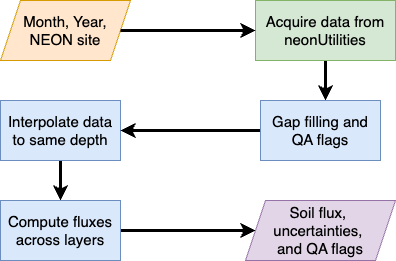
\includegraphics{figures/neonSoilFluxOutline.png}

}

\caption{\label{fig-package-diagram}Diagram of \texttt{neonSoilFlux} R
package. For a given month, year and NEON site (orange parallelogram),
the package acquires all relevant data to compute \(F_{S}\) using the
\texttt{neonUtilities} R package (green rectangle). Data are gap-filled
according to reported QA flags and interpolated to the same measurement
depth before computing the soil flux, uncertainties, and final QA flags
(blue rectangles). The package reports the associated soil flux,
uncertainties, and quality assurance (QA) flags for the user (purple
parallelogram).}

\end{figure}%

At a given NEON observation there are five replicate soil plots, each
with measurements of soil CO\(_{2}\) concentration, soil temperature,
and soil moisture at different depths (Figure~\ref{fig-model-diagram}).
The \texttt{neonSoilFlux} package acquires measured soil water content
(National Ecological Observatory Network (NEON), 2024e), soil CO\(_{2}\)
concentration (National Ecological Observatory Network (NEON), 2024b),
barometric pressure from the nearby tower (National Ecological
Observatory Network (NEON), 2024a), soil temperature (National
Ecological Observatory Network (NEON), 2024d), and soil properties
(e.g.~bulk density) (National Ecological Observatory Network (NEON),
2024c). The static soil properties were collected from a nearby soil pit
during site characterization and are assumed to be constant at each
site.

\begin{figure}

\centering{

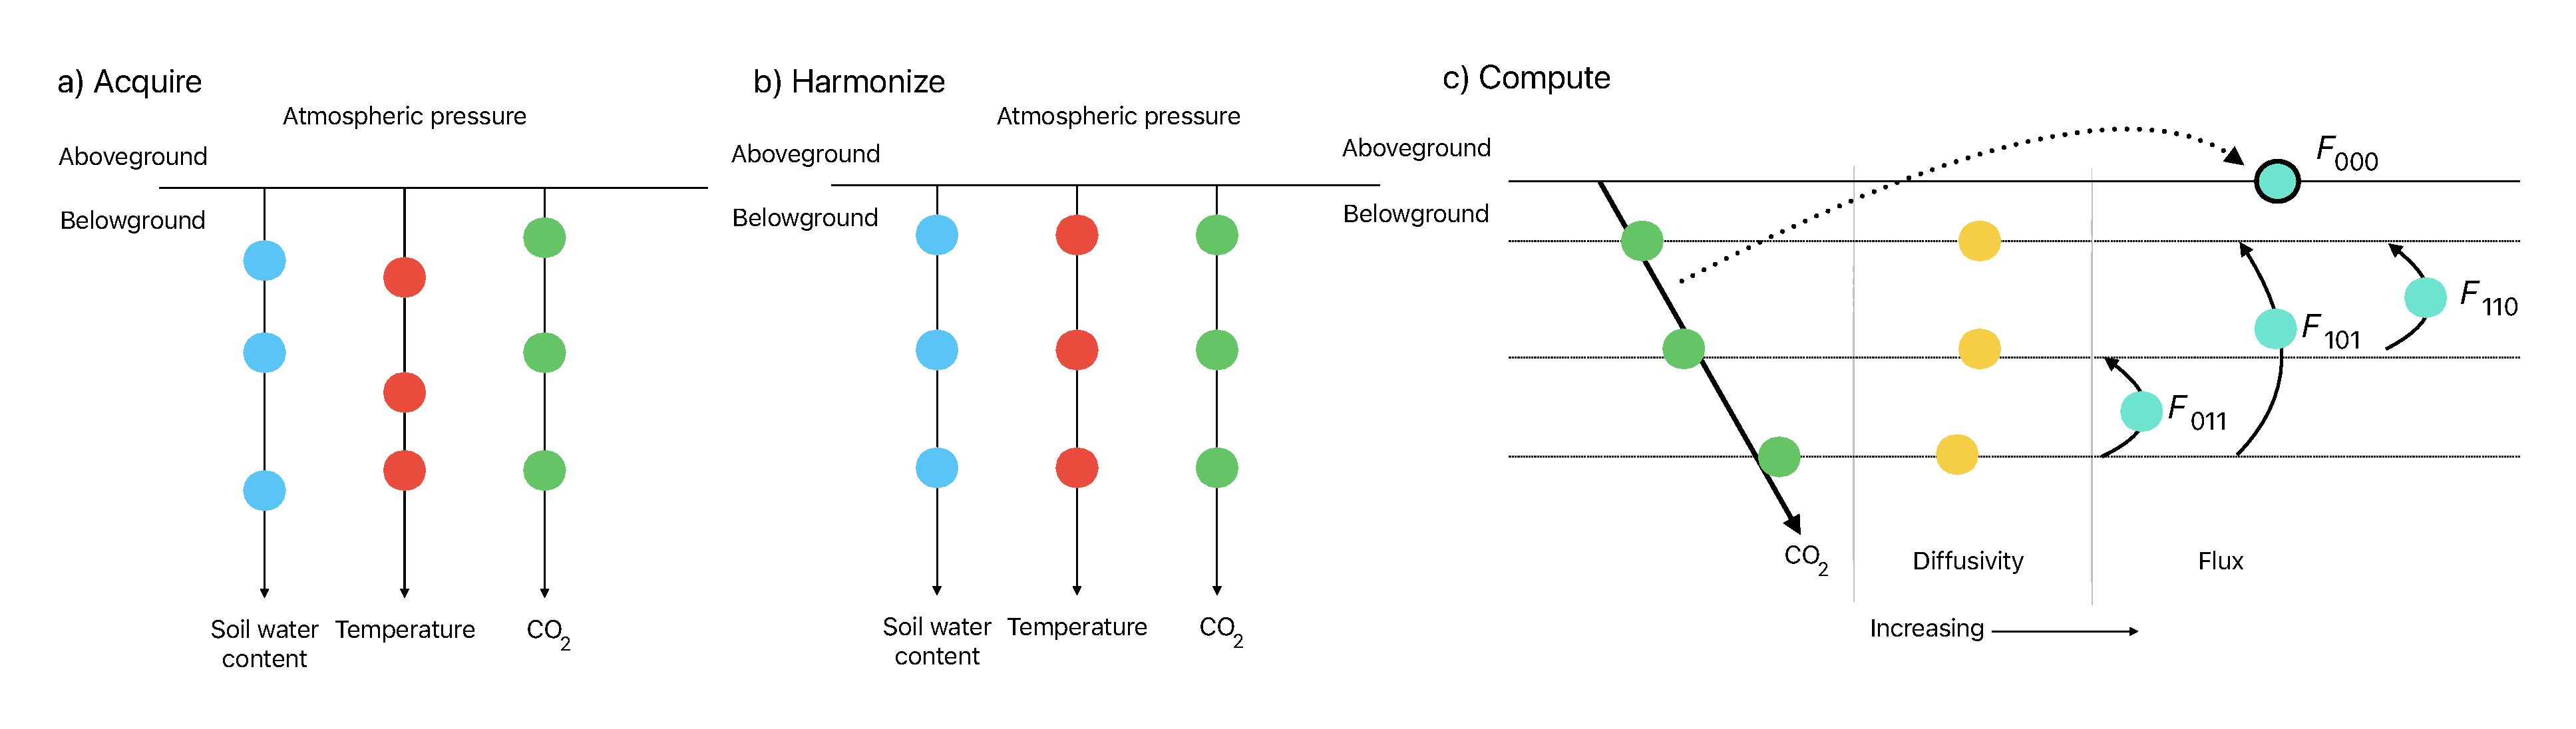
\includegraphics{figures/model-diagram.pdf}

}

\caption{\label{fig-model-diagram}Model diagram for data workflow for
the \texttt{neonSoilFlux} R package. a) Acquire: Data are obtained from
given NEON location and horizontal sensor location, which includes soil
water content, soil temperature, CO\(_{2}\) concentration, and
atmospheric pressure. All data are screened for quality assurance, with
gap-filling of missing data reported. b) Any belowground data are then
harmonized to the same depth as CO\(_{2}\) concentrations using linear
regression. c) The flux across a given depth is computed via Fick's law,
denoted with \(F_{ijk}\), where \(i\), \(j\), or \(k\) are either 0 or 1
denoting the layers the flux is computed across (\(i\) = closest to
surface, \(k\) = deepest). \(F_{000}\) represents a flux estimate where
the gradient \(dC/dz\) is the slope of a linear regression of CO\(_{2}\)
with depth.}

\end{figure}%

The workflow to computing a value of \(F_{S}\) with the
\texttt{neonSoilFlux} consists of three primary steps, illustrate in
Figure~\ref{fig-model-diagram}. First, NEON data are acquired for a
given site and month via the \texttt{neonUtilities} R package (yellow
parallelogram and green rectangle in Figure~\ref{fig-package-diagram}
and Panel a in Figure~\ref{fig-model-diagram}). Acquired environmental
data can be exported to a comma separated value file for additional
analysis. Quality assurance (QA) flags with an observation are reported
as an indicator variable.

The next step is harmonizing the data to compute soil fluxes across soil
layers. This step consists of three different actions (blue rectangles
in Figure~\ref{fig-package-diagram} and Panel b in
Figure~\ref{fig-model-diagram}). If a given observation by NEON is
reported as not passing a quality assurance check, we applied a gap
filling method to replace that measurement with its monthly mean at that
same depth (Section~\ref{sec-gapfilling}). Belowground measurements of
soil water and soil temperature are then interpolated to the same depth
as soil CO\(_{2}\) measurements. The diffusivity
(Section~\ref{sec-compute-diffusivity}) and soil flux across different
soil layers (Section~\ref{sec-compute-soil-flux}) are then computed.

The final step is computing a surface soil flux through extrapolation to
the surface (purple parallelogram in Figure~\ref{fig-package-diagram}
and Panel c in Figure~\ref{fig-model-diagram}). Uncertainty on a soil
flux measurement is computed through quadrature. An aggregate quality
assurance (QA) flag for each environmental measurement is also reported,
representing if any gap-filled measurements were used in the computation
of a soil flux. Within the soil flux-gradient method, several different
approaches can be used to derive a surface flux (Maier \&
Schack-Kirchner, 2014); the \texttt{neonSoilFlux} package reports four
different possible values of soil surface flux
(Section~\ref{sec-compute-soil-flux}).

\subsubsection{Gap-filling routine}\label{sec-gapfilling}

NEON reports QA flags as a binary value for a given measurement and
half-hourly time. We replaced any flagged measurements at a location's
spatial depth \(z\) with a bootstrapped sample of the monthly mean for
all un-flagged measurements for that month. These measurements are
represented by the vector \(\mathbf{m}\), standard errors
\(\boldsymbol\sigma\), and the 95\% confidence interval (the so-called
expanded uncertainty, Farrance \& Frenkel (2012))
\(\boldsymbol\epsilon\). All of these vectors have length \(M\). We have
that \(\vec{\sigma}_{i}\leq\vec{\epsilon}_{i}\). We define the bias as
\(\mathbf{b}=\sqrt{\boldsymbol\epsilon^{2}-\boldsymbol\sigma^{2}}\).

We generate a vector of bootstrap samples of the distribution of the
monthly mean \(\overline{\boldsymbol{m}}\) and monthly standard error
\(\overline{\boldsymbol\sigma}\) the following ways:

\begin{enumerate}
\def\labelenumi{\arabic{enumi}.}
\tightlist
\item
  Randomly sample from the uncertainty and bias independently:
  \(\boldsymbol\sigma_{j}\) and the bias \(\mathbf{b}_{k}\) (not
  necessarily the same sample).
\item
  Generate a vector \(\mathbf{n}\) of length \(N\), where
  \(\mathbf{n}_{i}\) is a random sample from a normal distribution with
  mean \(\boldsymbol{m}_{i}\) and standard deviation
  \(\boldsymbol\sigma_{j}\). Since \(M<N\), values from \(\mathbf{m}\)
  will be reused.
\item
  With these \(N\) random samples,
  \(\overline{y}_{i}=\overline{\vec{x}}+\vec{b}_{k}\) and \(s_{i}\) is
  the sample standard deviation of \(\vec{x}\). We expect that
  \(s_{i} \approx \vec{\sigma}_{j}\).
\item
  The reported monthly mean and standard deviation are then computed
  \(\overline{\overline{y}}\) and \(\overline{s}\). Measurements and
  uncertainties that did not pass the QA check are then substituted with
  \(\overline{\overline{y}}\) and \(\overline{s}\).
\end{enumerate}

This gap-filling method described here provides a consistent approach
for each data stream, however we recognize that other gap-filling
alternatives may be warranted for longer-term gaps (e.g.~such as
correlations with other NEON measurement levels and soil plots), or
measurement specific gap-filling routines. We discuss the effect of
gap-filling on our measurements in Section~\ref{sec-discussion}.

\subsubsection{Soil diffusivity}\label{sec-compute-diffusivity}

Soil diffusivity \(D_{a}\) at a given measurement depth is the product
of the diffusivity in free air \(D_{a,0}\) (m\(^{2}\) s\(^{-1}\)) and
the tortuosity \(\xi\) (no units) (Millington \& Shearer, 1971).

We compute \(D_{a,0}\) with Equation \ref{eq:da0}:

\begin{equation}
  D_{a,0} = 0.0000147 \cdot \left( \frac{T_{i} + 273.15}{293.15} \right)^{1.75} \cdot \left( \frac{P}{101.3} \right)
  \label{eq:da0}
\end{equation}

where \(T_{i}\) is soil temperature (\(^\circ\)C) at depth \(i\)
(National Ecological Observatory Network (NEON), 2024d) and \(P\)
surface barometric pressure (kPa) (National Ecological Observatory
Network (NEON), 2024a).

Previous studies by Sallam et al. (1984) and Tang et al. (2003)
demonstrated the sensitivity of modeled \(F_{S}\) depending on the
tortuousity model used to compute diffusivity. At low soil water
content, the choice of tortusoity model may lead to order of magnitude
differences in \(D_{a}\), which in turn affect modeled \(F_{S}\). The
\texttt{neonSoilFlux} package uses two different models for \(\xi\).
representing the extremes reported in Sallam et al. (1984). The first
approach uses the Millington-Quirk model for diffusivity, Equation
\ref{eq:tortuosity-mq} (Millington \& Shearer, 1971):

\begin{equation}
  \xi = \frac{(\phi - SWC_{i})^{10/3}}{\phi^{2}}
  \label{eq:tortuosity-mq}
\end{equation}

In Equation \ref{eq:tortuosity-mq}, \(SWC\) is the soil water content at
depth \(i\) (National Ecological Observatory Network (NEON), 2024e) and
\(\phi\) is the porosity (Equation \ref{eq:porosity}), which in turn is
a function of soil physical properties (National Ecological Observatory
Network (NEON), 2024c):

\begin{equation}
  \phi = \left(1- \frac{\rho_{s}}{\rho_{m}} \right) \left(1-f_{V}\right)
  \label{eq:porosity}
\end{equation}

In Equation \ref{eq:porosity}, \(\rho_{m}\) is the particle density of
mineral soil (2.65 g cm\(^{-3}\)), \(\rho_{s}\) the soil bulk density (g
cm\(^{-3}\)) excluding coarse fragments greater than 2 mm (National
Ecological Observatory Network (NEON), 2024c). The term \(f_{V}\) is a
site-specific value that accounts for the proportion of soil fragments
between 2-20 mm. Soil fragments greater than 20 mm were not estimated
due to limitations in the amount of soil that can be analyzed (National
Ecological Observatory Network (NEON), 2024c). We assume there are no
pores within rocks.

The second approach to calculate \(\xi\) is the Marshall model
(Marshall, 1959), where \(\xi = \phi^{1.5}\), with \(\phi\) defined from
Equation \ref{eq:porosity}.

\subsubsection{Soil flux computation}\label{sec-compute-soil-flux}

We applied Fick's law (Equation \ref{eq:ficks}) to compute the soil flux
\(F_{ij}\) (\(\mu\)mol m\(^{-2}\) s\(^{-1}\)) across two soil depths
\(i\) and \(j\):

\begin{equation}
  F_{ij} = -D_{a} \frac{dC}{dz}
  \label{eq:ficks}
\end{equation}

where \(D_{a}\) is the diffusivity (m\(^{2}\) s\(^{-1}\)) and
\(\frac{dC}{dz}\) is the gradient of CO\(_{2}\) molar concentration
(\(\mu\)mol m\(^{-3}\), so the gradient has units of \(\mu\)mol
m\(^{-3}\) m\(^{-1}\)). The soil surface flux is theoretically defined
by applying Equation \ref{eq:ficks} to measurements collected at the
soil surface and directly below the surface. Measurements of soil
temperature, soil water content, and soil CO\(_{2}\) molar concentration
across the soil profile allow for application of Equation \ref{eq:ficks}
across different soil depths. Each site had three measurement layers, so
we denote the flux between which two layers as a three-digit subscript
\(F_{ijk}\) with indicator variables \(i\), \(j\), and \(k\) indicate if
a given layer was used (written in order of increasing depth), according
to the following:

\begin{itemize}
\tightlist
\item
  \(F_{000}\) is a surface flux estimate using the intercept of the
  linear regression of \(D_{a}\) with depth and the slope from the
  linear regression of CO\(_{2}\) with depth (which represents
  \(\displaystyle \frac{dC}{dz}\) in Fick's Law). Tang et al. (2003)
  used this approach to compute fluxes in an oak-grass savannah.
\item
  \(F_{110}\), \(F_{011}\) are fluxes across the two most shallow layers
  and two deepest layers respectively. The diffusivity used in Fick's
  Law is always at the deeper measurement layer. When used as a surface
  flux estimate we assume CO\(_{2}\) remains constant above this flux
  depth.
\item
  \(F_{101}\) is a surface flux estimate using linear extrapolation
  using concentration measurements between the shallowest and deepest
  measurement layer. Hirano et al. (2003) and Tang et al. (2005) used an
  approach similar to \(F_{101}\) in a temperate deciduous broadleaf
  forest and ponderosa pine forest respectively.
\end{itemize}

Uncertainty in all \(F_{ijk}\) is computed through quadrature (Taylor,
2022).

\subsection{Post processing evaluation}\label{sec-post-process}

Following collection of field measurements from the LICOR and
calculation of the soil fluxes from \texttt{neonSoilFlux} package, we
compared measured \(F_{S}\) (from the LICOR instruments) to a given soil
flux calculation \texttt{neonSoilFlux} for each site and flux
computation method. Statistics included the associated R\(^{2}\) value,
root mean squared error (RMSE), and signal to noise ratio (SNR), defined
as the ratio of a modeled soil flux (\(F_{ijk}\)) from
\texttt{neonSoilFlux} to its quadrature uncertainty (\(\sigma_{ijk}\)).

We observed that the range of values (e.g.~\(F_{ijk} \pm \sigma_{ijk}\)
was much larger than the measured field flux. We evaluated
\(| F_{S} - F_{ijk} | < (1-\epsilon) \sigma_{ijk}\), where \(F_{S}\) is
a measured field soil flux from the LICOR 6800 (the LICOR 8250 was used
at only three sites). The parameter \(\epsilon\) was an uncertainty
reduction factor to evaluate how much the quadrature uncertainty could
be reduced while maintaining precision between modeled \(F_{ijk}\) and
measured \(F_{S}\).

Finally, for a half-hourly interval we also computed a \emph{post hoc}
\(D_{a}\) using the LICOR flux along with the CO\(_{2}\) surface
gradient reported by NEON using the measurement levels closest to the
surface.

\section{Results}\label{results}

Figure~\ref{fig-flux-results} reports the timeseries of out the measured
fluxes from the LICOR 6800 and 8250 compared to modeled soil fluxes from
the \texttt{neonSoilFlux} R package. Figure~\ref{fig-flux-results-year}
and and computed fluxes and uncertainty at each measurement site.
Results are reported in local time. Positive values of the flux indicate
that there is a flux moving towards the surface. For ease of clarity the
fluxes at \(F_{111}\) and \(F_{000}\) are only shown in the top row
(surface), followed by the fluxes at individual separate layer
(\(F_{100}\), \(F_{010}\), \(F_{001}\)). Overall, with the exception of
WREF and SRER (discussed later) the computed fluxes were on the same
order of magnitude and timing as the measured field fluxes.

\begin{figure}

\centering{

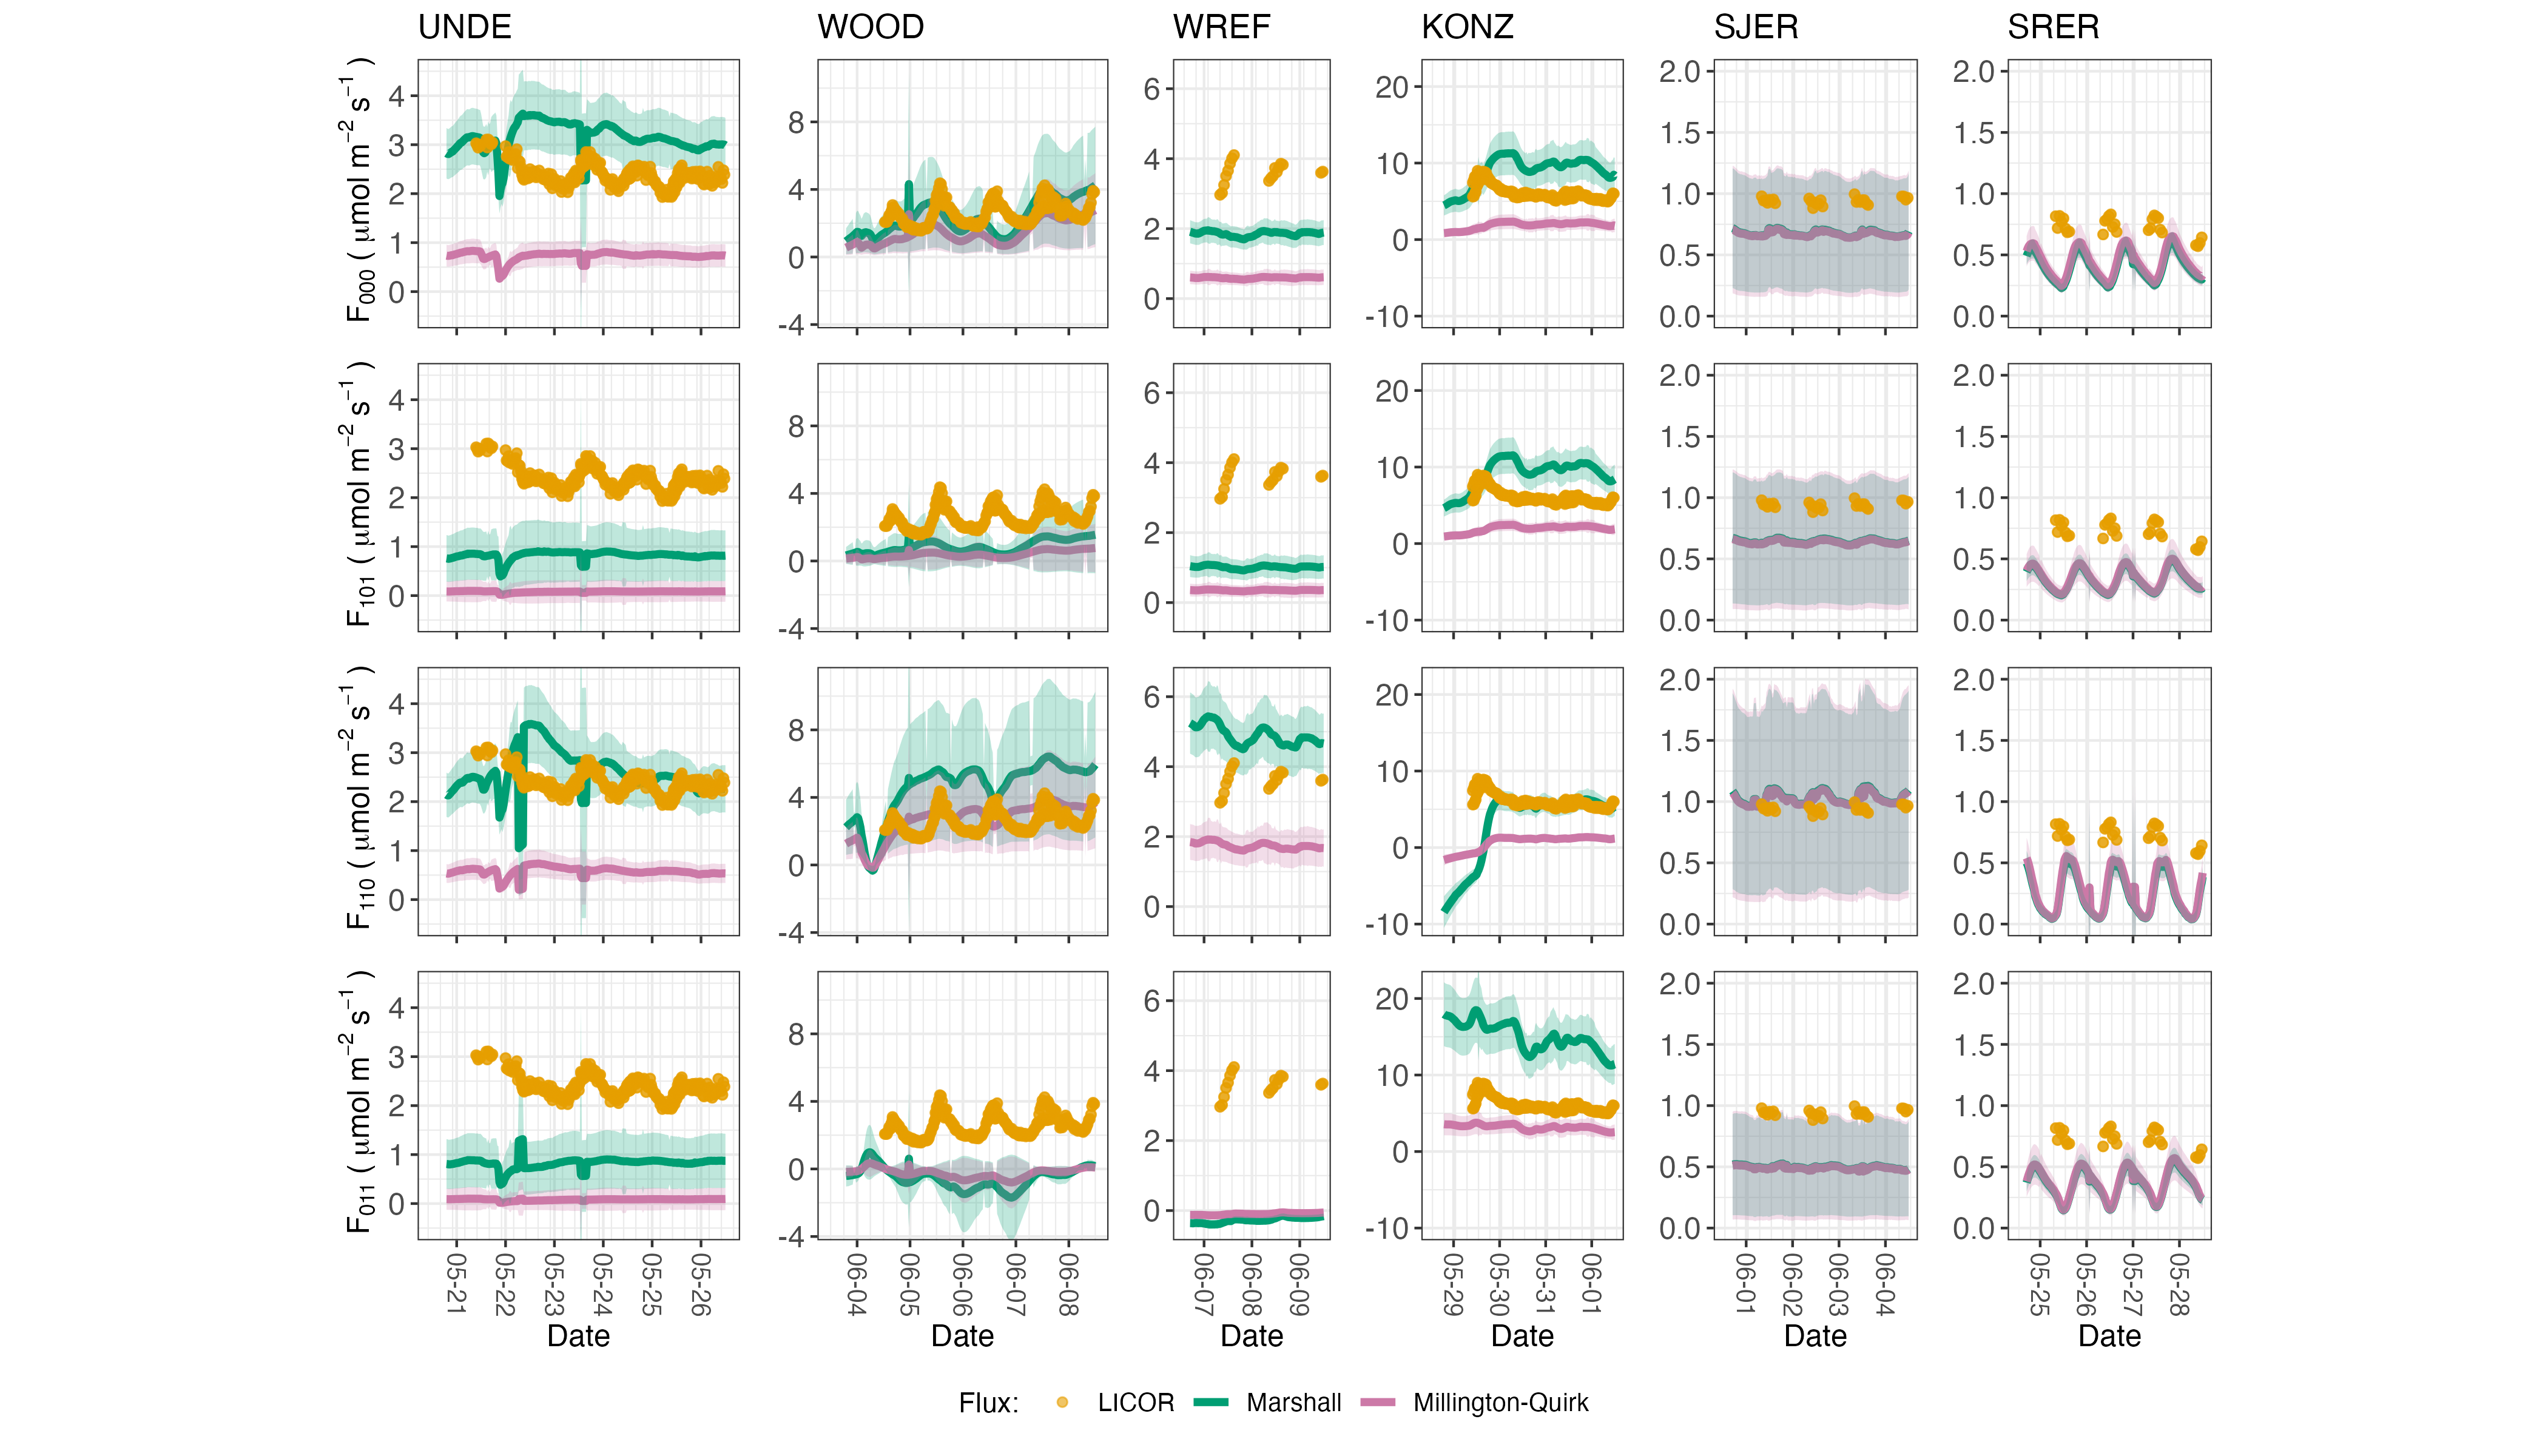
\includegraphics{figures/flux-results.png}

}

\caption{\label{fig-flux-results}Timeseries of both measured \(F_{S}\)
(yellow circles) and modeled soil fluxes (green or purple lines) by the
\texttt{neonSoilFlux} R package. Fluxes from the \texttt{neonSoilFlux} R
package are separated by the diffusivity model used (Millington-Quirk or
Marshall, Section~\ref{sec-compute-diffusivity}). Vertical axis labels
in the first column represent the measurement levels where the
flux-gradient approach is applied (Section~\ref{sec-compute-soil-flux}).
Ribbons for modeled soil fluxes represent \(\pm\) 1 standard deviation.
Results are reported in local time.}

\end{figure}%

\begin{figure}

\centering{

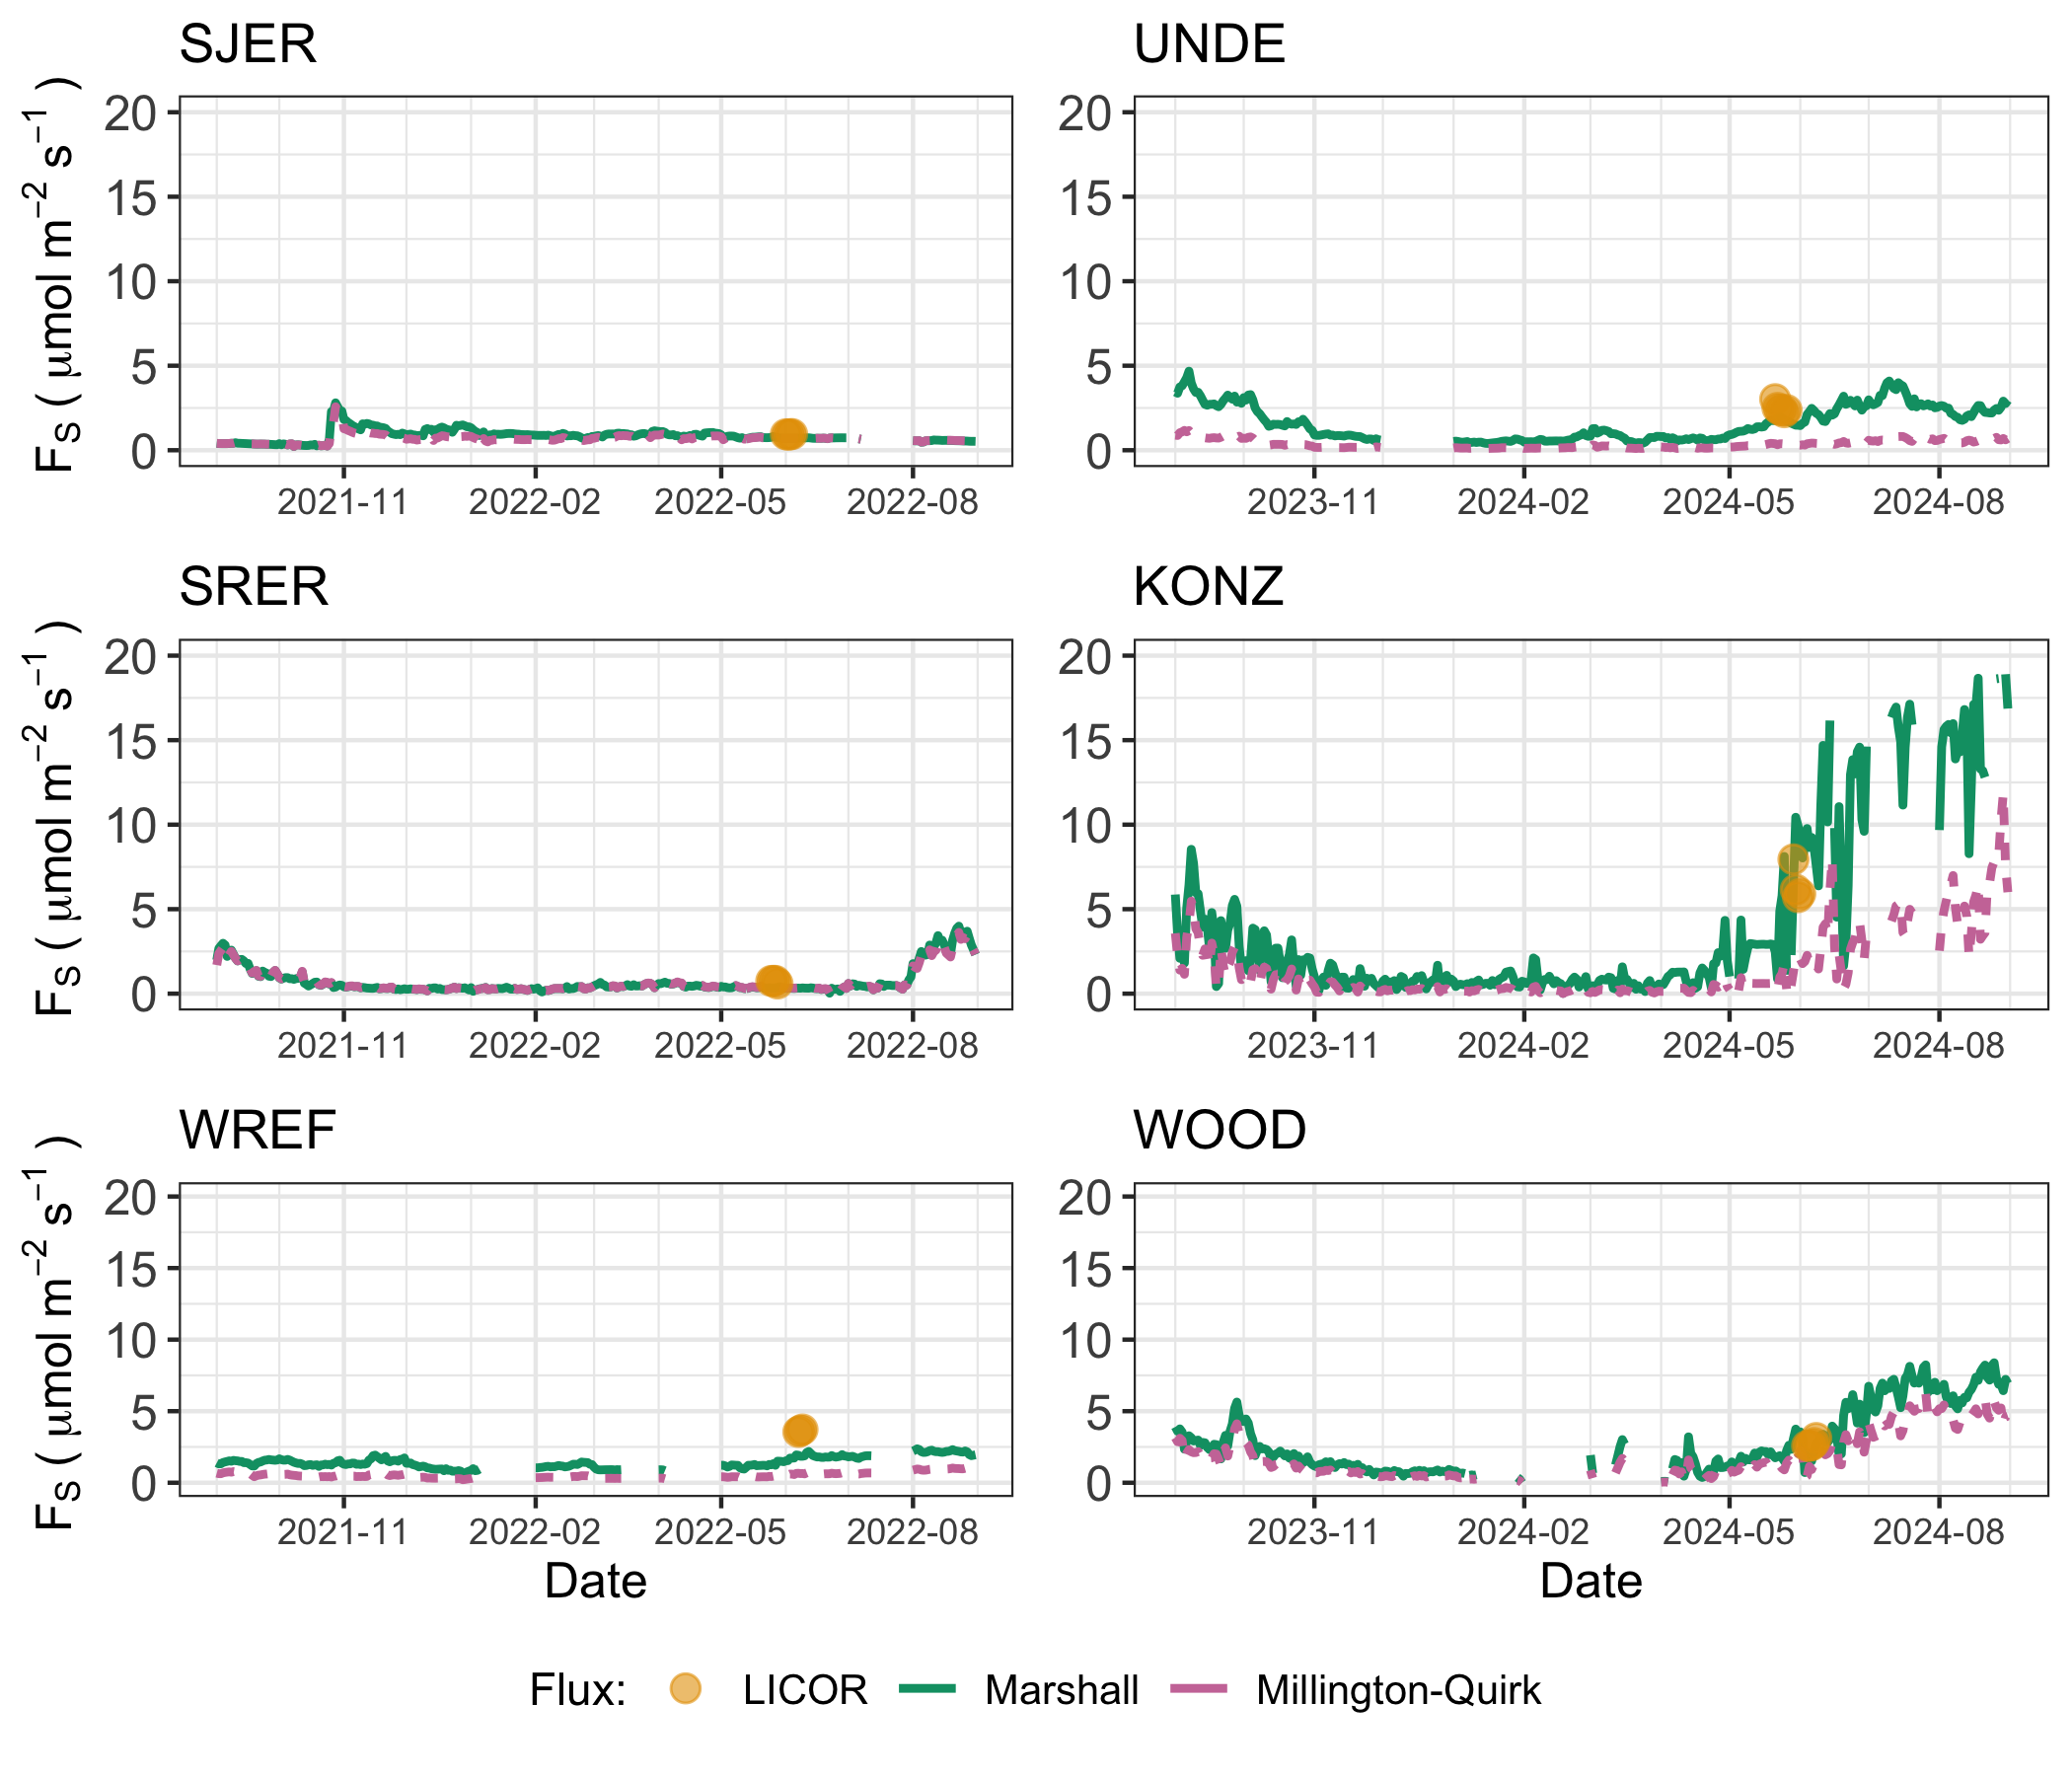
\includegraphics{figures/flux-results-year.png}

}

\caption{\label{fig-flux-results-year}Timeseries of both daily-averaged
field \(F_{S}\) (yellow circles) and daily ensemble averaged soil fluxes
(green or purple lines) by the \texttt{neonSoilFlux} R package,
separated by the diffusivity model used (Millington-Quirk or Marshall,
Section~\ref{sec-compute-diffusivity}). The timeseries of modeled fluxes
are a daily ensemble average of all flux-gradient approaches
(\(F_{000}\), \(F_{101}\), \(F_{011}\), \(F_{110}\),
Section~\ref{sec-compute-soil-flux}).}

\end{figure}%

\begin{figure}

\centering{

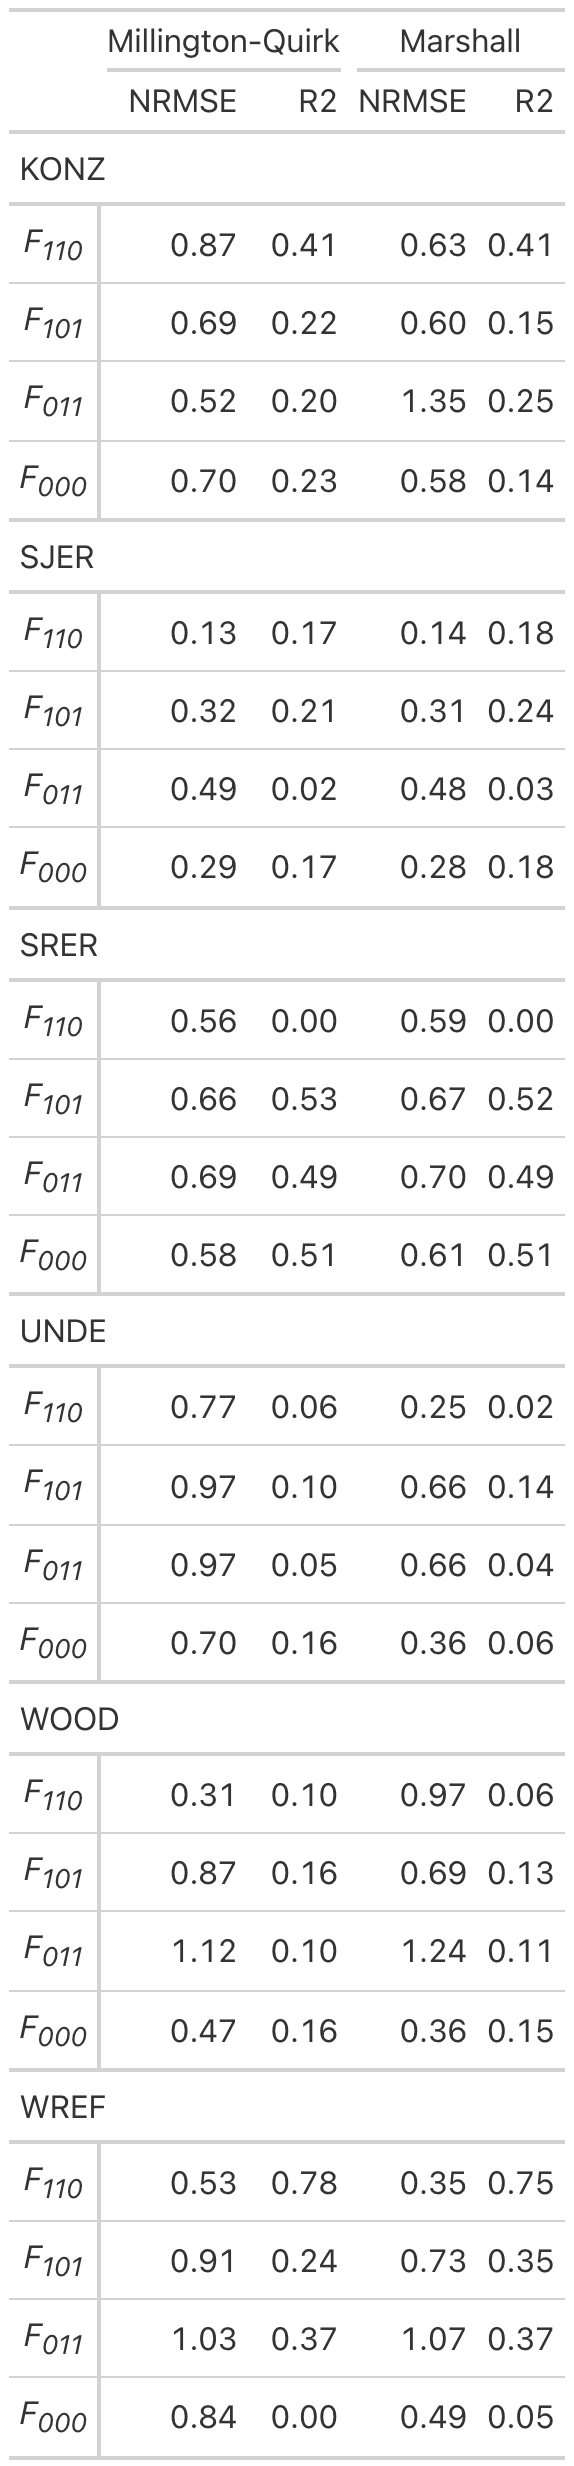
\includegraphics{figures/r2-plot.png}

}

\caption{\label{fig-r2-table}}

\end{figure}%

For a given half-hourly time period, the \texttt{neonSoilFlux} packages
assigns a QA flag for a measurement if more one values across all
measurement depths uses gap-filled data (Section~\ref{sec-gapfilling}).
Panel a of Figure~\ref{fig-gap-filled-stats} reports the distribution
for all input environmental measurements at each site when field
measurements were made. Soil fluxes are computed from 4 different types
of input measurements (\(T_{S}\), \(SWC\), \(P\), and CO\(_{2}\)), any
of which could have a QA flag in a half-hourly interval. Panel b of
Figure~\ref{fig-gap-filled-stats} displays at each site the distribution
of the number of different gap-filled measurements used to compute a
half-hourly flux. The largest contribution to gap-filled measurements
was soil water. SJER and WOOD utilized the largest number of gap-filled
measurements, which were primarily \(SWC\) and \(T_{S}\).

\begin{figure}

\centering{

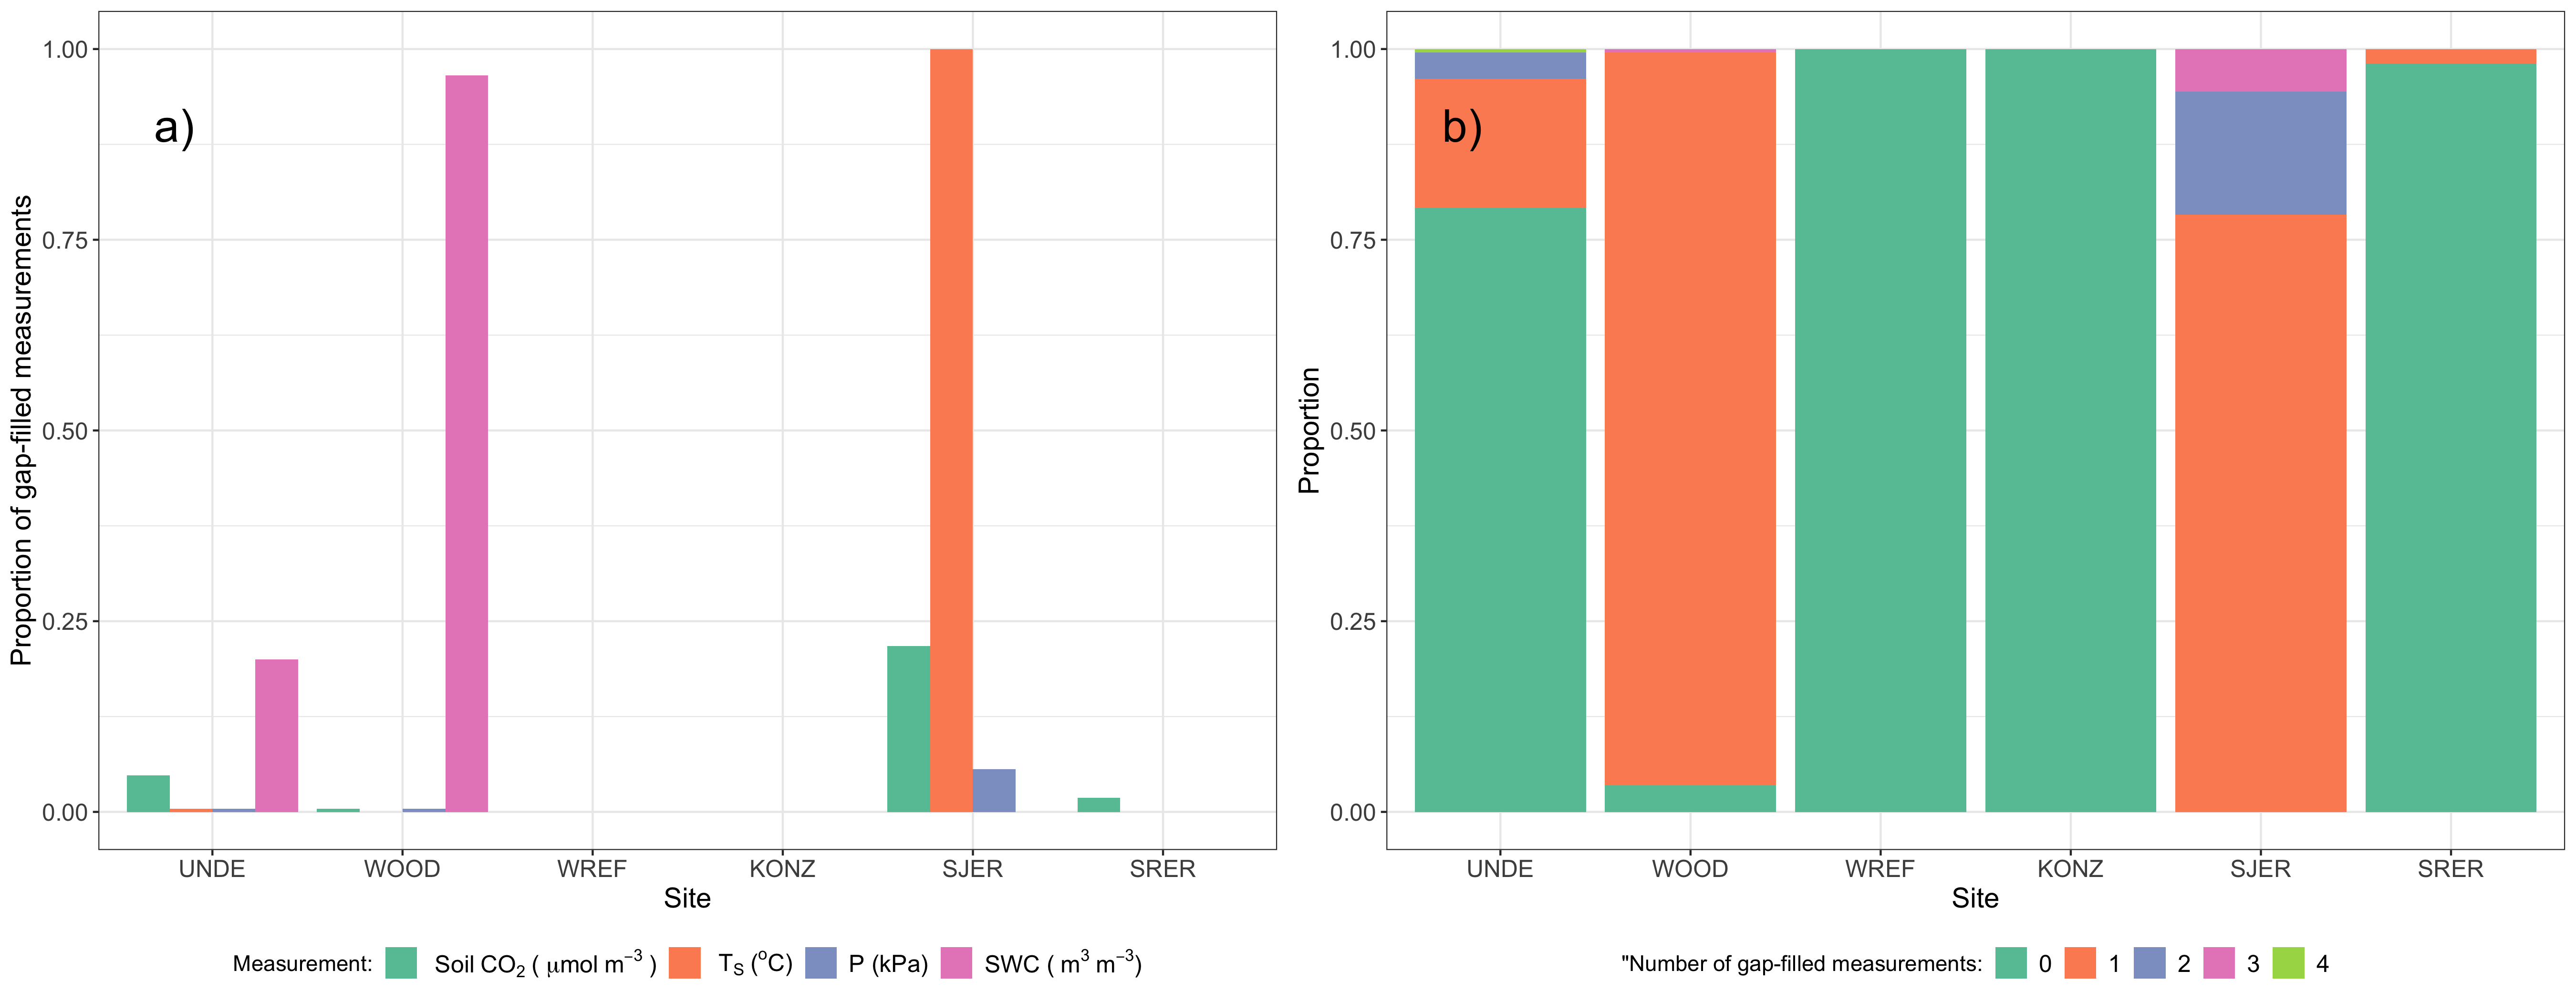
\includegraphics{figures/gap-filled-stats.png}

}

\caption{\label{fig-gap-filled-stats}Panel a) Proportion of input
gap-filled environmental measurements used to generate \(F_{S}\) from
the \texttt{neonSoilFlux} package, by study site. Panel b) distribution
of the usage of gap-filled measurements at each site.}

\end{figure}%

Figure~\ref{fig-uncertainty-stats} reports both the computed SNR and the
proportion of measured field fluxes within the modeled uncertainty for a
given flux computation method \(F_{ijk}\)
(Section~\ref{sec-post-process}). Here, values of SNR greater than unity
indicates a reported uncertainty is smaller, propogated by quadrature
from a relatively higher precision from measured input variables
(CO\(_{2}\), \(T_{S}\), \(SWC\), or \(P\)). The sensitivity to the
uncertainty reduction factor (\(\epsilon\), bottom panels in
Figure~\ref{fig-uncertainty-stats}) demonstrates how accuracy could be
improved if modeled uncertainty \(\sigma_{ijk}\) decreases.

\begin{figure}

\centering{

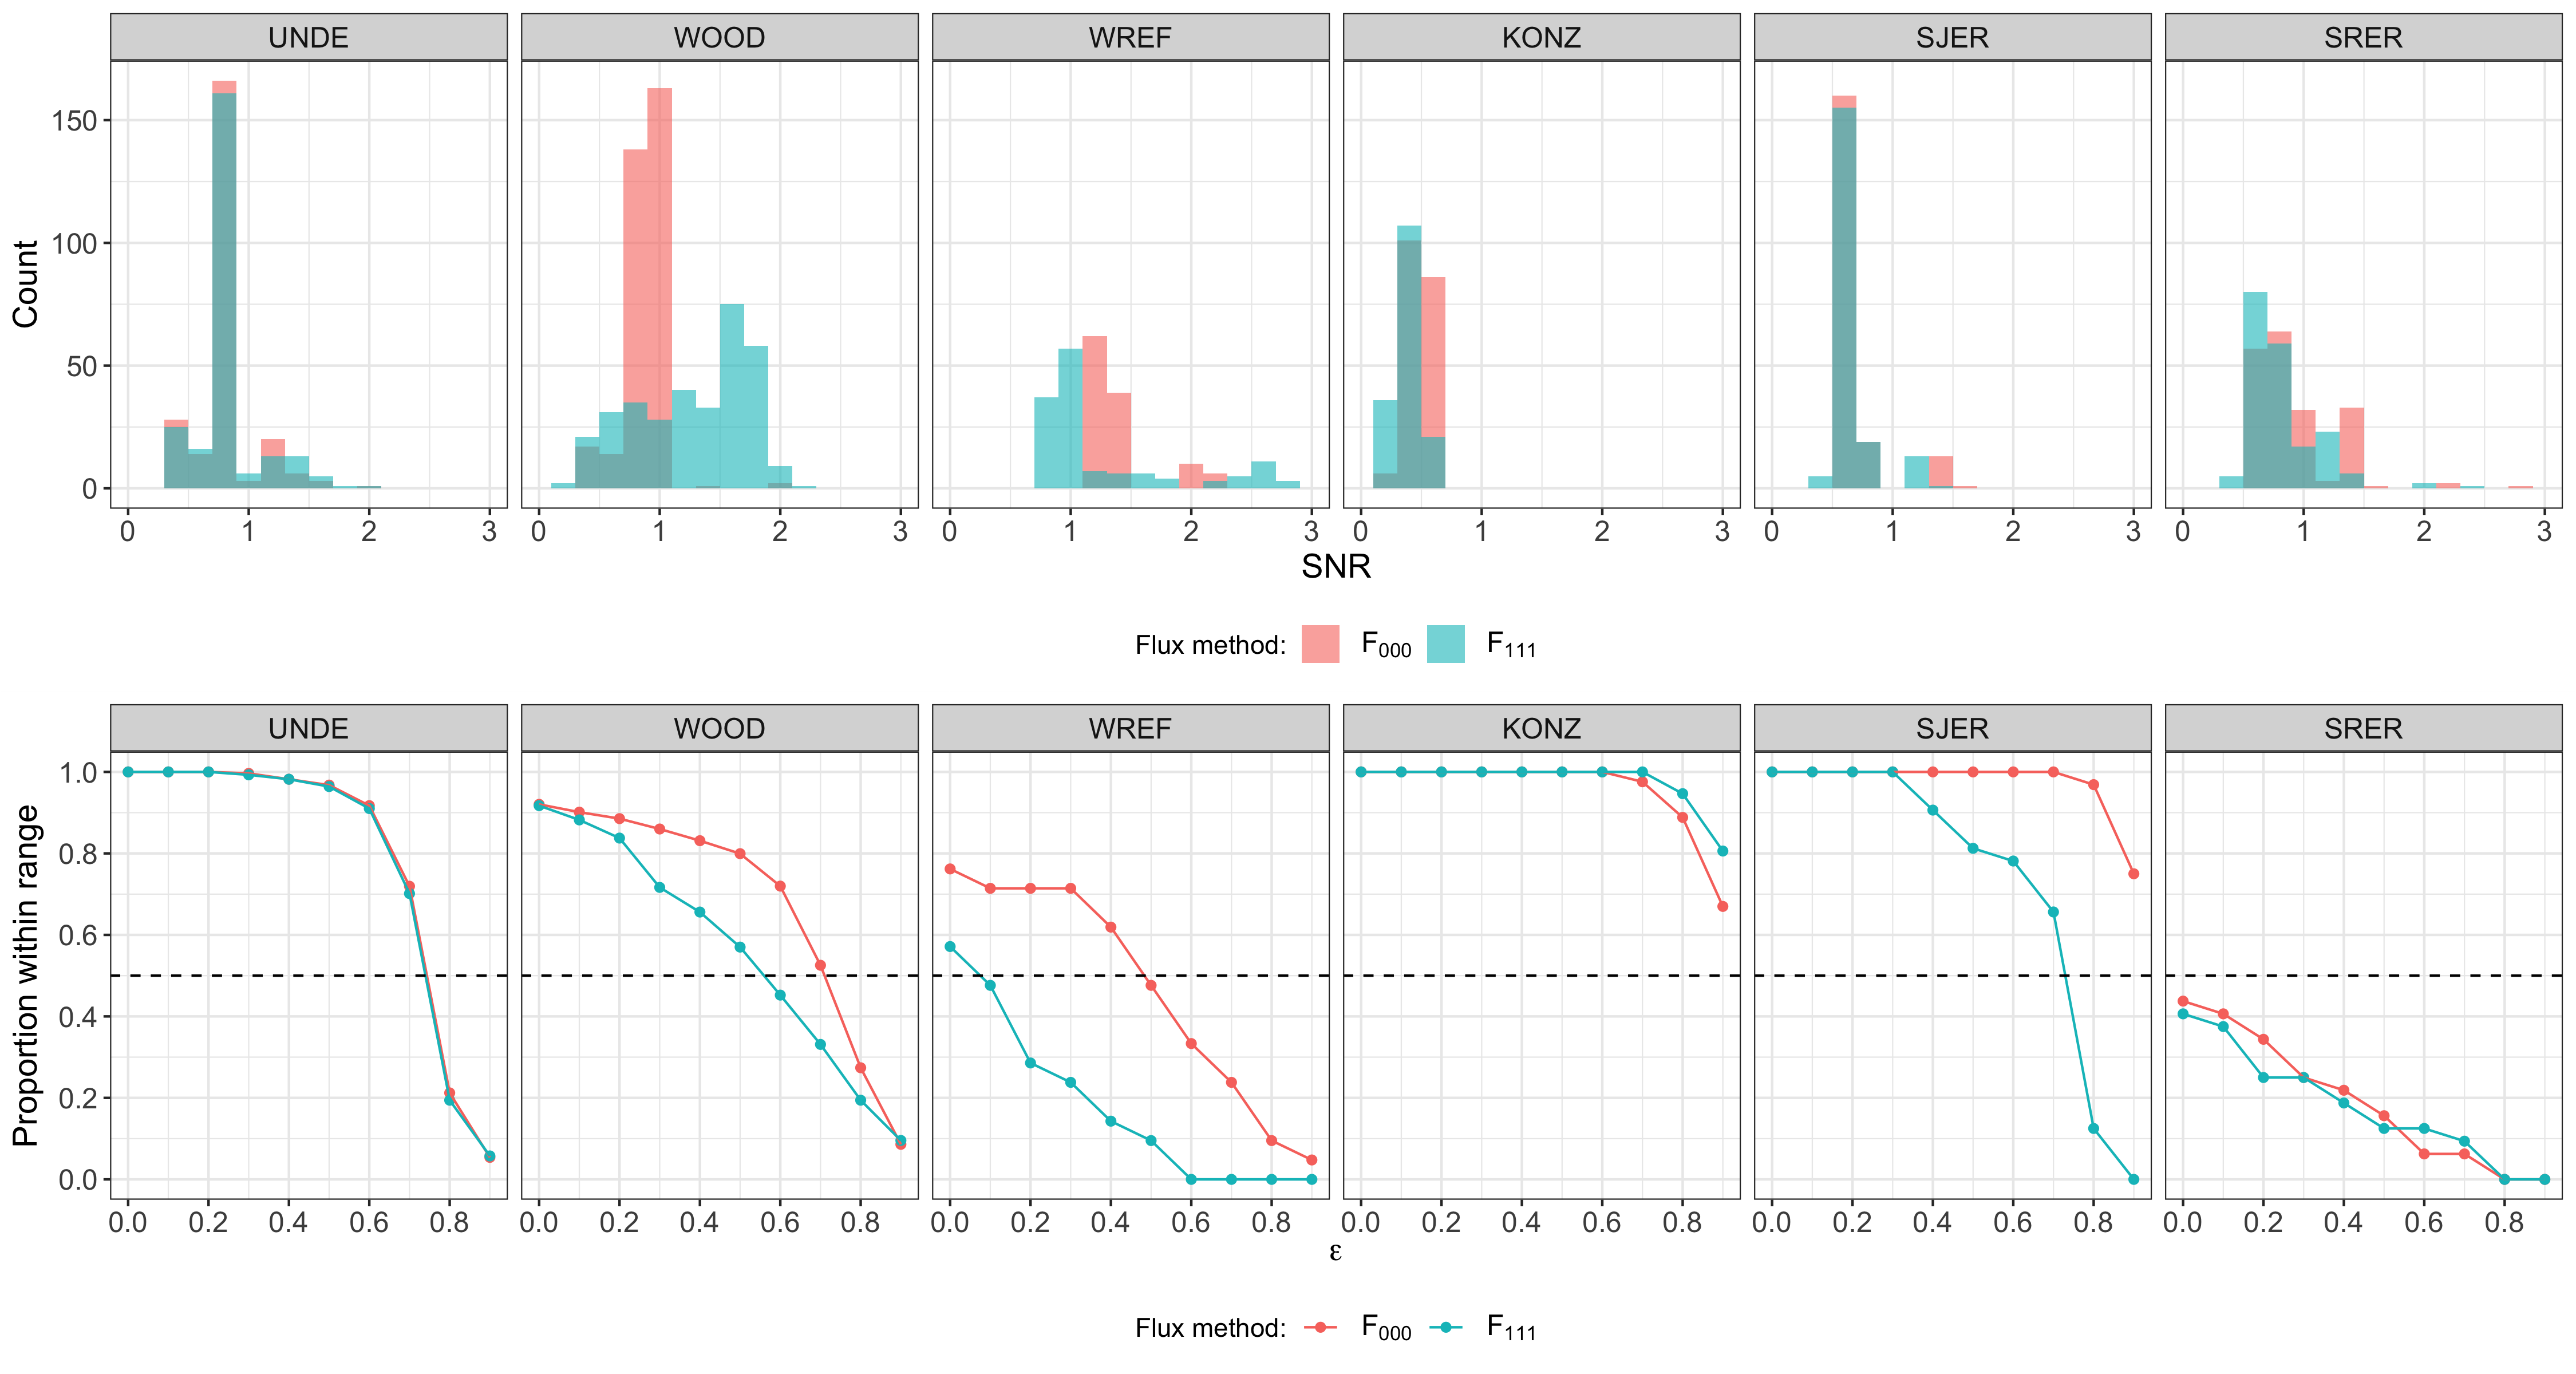
\includegraphics{figures/uncertainty-stats.png}

}

\caption{\label{fig-uncertainty-stats}Top panels: distribution of SNR
values across each of the different sites for modeled effluxes from the
\texttt{neonSoilFlux} package, depending on the diffusivity calculation
used (Millington-Quirk or Marshall,
Section~\ref{sec-compute-diffusivity}). Bottom panels: Proportion of
measured \(F_{S}\) within the modeled range of a flux computation method
\(F_{ijk}\) given an uncertainty reduction factor \(\epsilon\), or
\(| F_{S} - F_{ijk} | < (1-\epsilon) \sigma_{ijk}\).}

\end{figure}%

Figure~\ref{fig-diffusivity-plot} reports the distribution of \(D_{a}\)
(from both the Marshall and Millington-Quirk methods,
Section~\ref{sec-compute-diffusivity}) at each study site, and the
\emph{post hoc} computation of \(D_{a}\)
(Section~\ref{sec-compute-diffusivity}).

\begin{figure}

\centering{

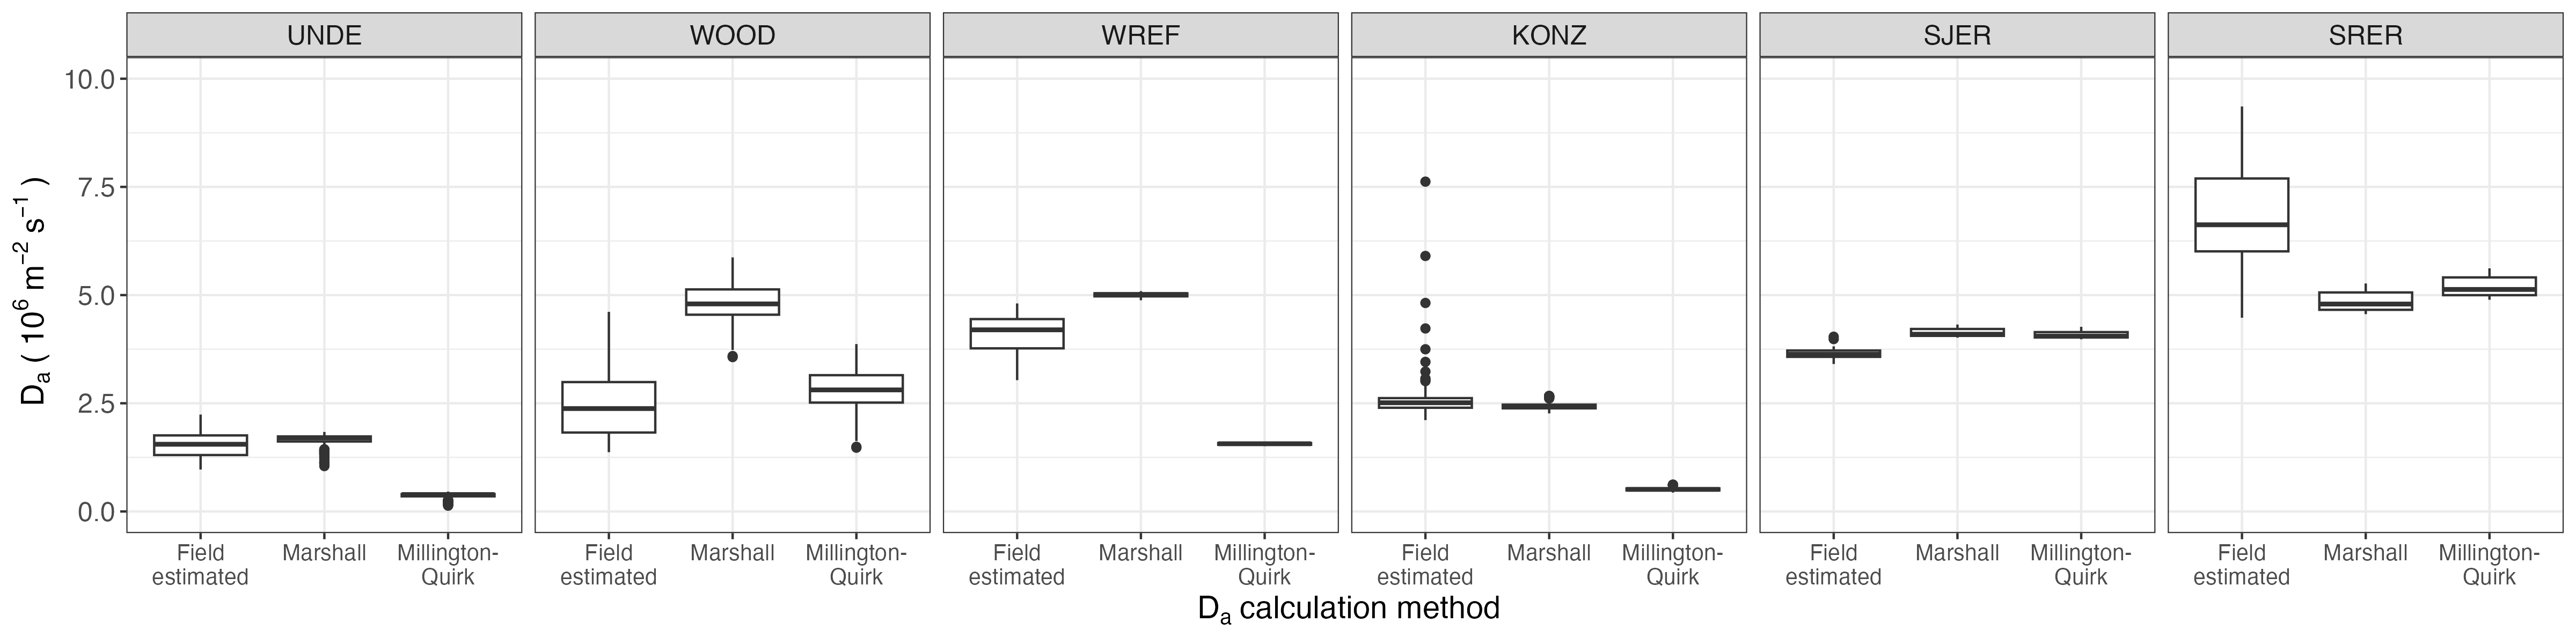
\includegraphics{figures/diffusivity-plot.png}

}

\caption{\label{fig-diffusivity-plot}}

\end{figure}%

\section{Discussion}\label{sec-discussion}

This study presents a unified data science workflow to efficiently
process automated measurements of belowground soil CO\(_{2}\)
concentrations, water, and temperature to infer estimates of soil
surface CO\(_{2}\) effluxes through application of Fick's Law (Equation
\ref{eq:ficks}). Our core goals in this study were: (1) to generate
estimates of soil flux from continuous soil sensor data at terrestrial
NEON sites using the flux-gradient method and then (2) to compare those
estimates to field-measured fluxes based on the closed chamber approach
at six NEON focal sites. We discuss our progress toward these core goals
through (1) an overall evaluation of the flux-gradient approach (and
uncertainty calculation) and (2) site-specific evaluation of differences
in estimated vs measured fluxes.

\subsection{General evaluation of flux-gradient
approach}\label{general-evaluation-of-flux-gradient-approach}

Key assumptions of the flux-gradient approach are that CO\(_{2}\)
concentrations increase throughout the soil profile. We found that this
condition was met at XXX\% across the study period. Periods where this
gradient condition are not met generally are connected to biophysical
processes such soil wetting events (e.g.~KONZ), which have the effect of
reducing the soil respiration or efflux due to a temporary reduction in
diffusivity. When modeling soil respiration, typically a non-linear
response function that also considers soil type is used (Bouma \& Bryla,
2000; Yan et al., 2016, 2018). For the \texttt{neonSoilFlux} package,
soil type is connected to the bulk density, which was characterized at
each NEON site based on replicate samples collected from the site
megapit at a subset of soil horizons, with an estimated uncertainty of
\(\pm5\%\) (see NEON User Guide to Soil physical and chemical
properties, Megapit (DP1.00096.001)). Coarse fragment estimates also
have very large uncertainties, but because the volume fraction tends to
be low in surface soils it probably wouldn't contribute much additional
flux uncertainty.

The largest source of uncertainty to improve reliability of the flux
estimate is to prevent the usage of gap-filled data. Three sites (KONZ,
SRER, and KONZ) had more than 75\% of half-hourly periods with no-gap
filled measurements. Two sites (SJER and WOOD) had more than 75\% of
half-hourly intervals with just one gap-filled measurement. While WREF
reported no gap-filled measurements, field data collection occurred
following a once-in-a century rainstorm with soils observed at their
water holding capacity. We recommend that whenever available, local
field knowledge is supplementary to any QA filtering protocol of fluxes
from the \texttt{neonSoilFlux} package.

We recognize that this gap-filling approach may lead to gap-filled
values that are quite different from the actual values, such as an
underestimate of soil moisture following rain events. Further extensions
of the gap filling method could use more sophisticated gap-filling
routines, similar to what is used for net ecosystem carbon exchange
(Falge et al., 2001; Liu et al., 2023; Mariethoz et al., 2015; Moffat et
al., 2007; Zhang et al., 2023). The current gap-filling routine provides
a consistent approach that can be applied to each data stream, but
further work may explore alternative gap-filling approaches.

Based on this approach, we would \emph{a priori} expect
\(F_{011} \leq F_{101} \leq \leq F_{110} \leq F_{000}\) because the
previous flux estimates ones correspond to deeper depths which will
could miss CO\(_{2}\) produced in shallower layers. Additionally, field
flux measurements should correlate with \(F_{000}\) because they
represent surface fluxes.

\subsection{Evaluation of flux-gradient approach at each
site}\label{evaluation-of-flux-gradient-approach-at-each-site}

Derived results from the \texttt{neonSoilFlux} package have patterns
that are consistent, and comparable, to those directly measured to the
field (Figure XXX). The advantage to the \texttt{neonSoilFlux} package
is the calculation of fluxes across different measurement depths,
allowing for additional site-specific customization. Here application of
the flux-gradient method provides a baseline estimate of soil fluxes
that could be complemented through additional field measurements
(e.g.~LICOR).

The six sites studied provide separate case studies for considerations
when applying the flux-gradient method to evaluate resulting
uncertainties and fluxes For example, SRER is characterized by sandy
soil, which also led to the highest observed field soil temperatures. At
SRER the flux across the top two layers (\(F_{110}\)) produced a pattern
of soil flux consistent with the observed field data. The remaining
methods \(F_{101}\), \(F_{011}\), or \(F_{000}\) are derived from
information at the deeper layer, which is decoupled both in terms of
temperature and CO\(_{2}\) concentration.

In addition, KONZ is a site that experienced a significant rain event
prior to sampling with eventual drying out over the course of the
experiment. In this case we observed storage of soil water which
increased the soil CO\(_{2}\) at the top layer, leading to negative
values of flux at the start of the experiment, with the fluxes drying
out afterwards. In this case only when the soil dried out (or returned
to a baseline level), that the fluxes at the provided layer would work
out in this case.

When considering systematic deployment of this method across a
measurement network, we faced a number of independent challenges for
consideration.

Figure~\ref{fig-uncertainty-stats} illustrates the tradeoff between
accuracy for modeled fluxes (defined here as closeness to field-measured
\(F_{S}\)) and precision defined by the SNR, and how this is confounded
by the choice of diffusivity model used. MORE HERE

Diffusivity discussion

In developing and validating our approach, we faced a number of
challenges related to data availability, including\ldots{} gap filling,
sensor calibration, depth interpolation, rainstorms, etc These errors
are all

\subsection{Recommendations for future method
development}\label{recommendations-for-future-method-development}

The \texttt{neonSoilFlux} package provides three different approaches of
values for a soil flux. We believe these approaches reflect a variety of
site-specific determination and assumptions used to generate a soil flux
measurement (Maier \& Schack-Kirchner, 2014), with the choice of method
having a determinative approach on reported values. Reported results
could further be distilled down using ensemble averaging averaging
approaches (Elshall et al., 2018; Raftery et al., 2005).

Figures XXX suggests that the provided uncertainty from
\texttt{neonSoilFlux} is an overestimate compared to what is actually
computed. When \(\epsilon=0\) in Figure
Figure~\ref{fig-uncertainty-stats}, that means we are just using the
reported uncertainty from neonSoilFlux. Looking at that (epsilon = 0)
shows field measurements UNDE, KONZ, SJER are 100\% within the reported
intervals from neonSoilFlux. But those sites tend to have a SNR
\textless{} 1, so the uncertainty is pretty noisy. For UNDE, we could
even reduce the uncertainty by a factor of 75\% (epsilon = 0.75), more
than half of the field measurements will still be within the reported
intervals. For KONZ, we are still within 70\% of the reported intervals
when uncertainty is reduced by 90\%. That suggests that while the
reported accuracy (as compared to field measurements), we do have higher
precision.

These challenges notwithstanding, the method used here and made
available in the \texttt{neonSoilFlux} R package has the potential to
produce nearly continuous estimates of flux across all terrestrial NEON
sites. These estimates are a significant improvement on available
approaches to constrain the portion of ecosystem respiration
attributable to the soil. This, in turn, aids in our ability to
understand the components of net ecosystem flux assessed at these sites
using the co-located eddy flux towers.

\begin{itemize}
\tightlist
\item
  Refine estimates to provide a realistic constraint on surface
  concentration measurements, thereby increasing the gradient.
\item
  Apply machine learning algorithms (e.g.~random trees) or model
  averaging techniques to generate a single flux estimate across each
  sites spatial location
\item
  Benchmarking flux results to estimates provided by Net ecosystem
  carbon exchange.
\end{itemize}

\section{Conclusions}\label{conclusions}

We have here presented an R package \texttt{neonSoilFlux} for the
estimation of soil CO\(_{2}\) fluxes from continuous buried soil sensor
measurements across terrestrial National Ecological Observatory Network
sites. We compared the predicted fluxes to those measured directly using
a field-based closed chamber approach. We find that\ldots{}

\phantomsection\label{refs}
\begin{CSLReferences}{1}{0}
\bibitem[\citeproctext]{ref-baldocchiMeasuringFluxesTrace2014}
Baldocchi, D. (2014). Measuring fluxes of trace gases and energy between
ecosystems and the atmosphere - the state and future of the eddy
covariance method. \emph{Global Change Biology}, \emph{20}(12),
3600--3609. \url{https://doi.org/10.1111/gcb.12649}

\bibitem[\citeproctext]{ref-berenbaumReportNSFBIO2015}
Berenbaum, M. R., Carpenter, S. R., Hampton, S. E., Running, S. W., \&
Stanzione, D. C. (2015). \emph{Report from the {NSF BIO Advisory
Committee Subcommittee} on {NEON Scope Impacts}}.

\bibitem[\citeproctext]{ref-bond-lambertyNewTechniquesData2018}
Bond-Lamberty, B. (2018). New {Techniques} and {Data} for
{Understanding} the {Global Soil Respiration Flux}. \emph{Earth's
Future}, \emph{6}(9), 1176--1180.
\url{https://doi.org/10.1029/2018EF000866}

\bibitem[\citeproctext]{ref-bond-lambertyTwentyYearsProgress2024}
Bond-Lamberty, B., Ballantyne, A., Berryman, E., Fluet-Chouinard, E.,
Jian, J., Morris, K. A., Rey, A., \& Vargas, R. (2024). Twenty {Years}
of {Progress}, {Challenges}, and {Opportunities} in {Measuring} and
{Understanding Soil Respiration}. \emph{Journal of Geophysical Research:
Biogeosciences}, \emph{129}(2), e2023JG007637.
\url{https://doi.org/10.1029/2023JG007637}

\bibitem[\citeproctext]{ref-bond-lambertyCOSORECommunityDatabase2020}
Bond-Lamberty, B., Christianson, D. S., Malhotra, A., Pennington, S. C.,
Sihi, D., AghaKouchak, A., Anjileli, H., Altaf Arain, M., Armesto, J.
J., Ashraf, S., Ataka, M., Baldocchi, D., Andrew Black, T., Buchmann,
N., Carbone, M. S., Chang, S.-C., Crill, P., Curtis, P. S., Davidson, E.
A., \ldots{} Zou, J. (2020). {COSORE}: {A} community database for
continuous soil respiration and other soil-atmosphere greenhouse gas
flux data. \emph{Global Change Biology}, \emph{26}(12), 7268--7283.
\url{https://doi.org/10.1111/gcb.15353}

\bibitem[\citeproctext]{ref-bond-lambertyGlobalDatabaseSoil2010}
Bond-Lamberty, B., \& Thomson, A. (2010). A global database of soil
respiration data. \emph{Biogeosciences}, \emph{7}(6), 1915--1926.
\url{https://doi.org/10.5194/bg-7-1915-2010}

\bibitem[\citeproctext]{ref-bond-lambertyGlobalRelationshipHeterotrophic2004}
Bond-Lamberty, B., Wang, C., \& Gower, S. T. (2004). A global
relationship between the heterotrophic and autotrophic components of
soil respiration? \emph{Global Change Biology}, \emph{10}(10),
1756--1766. \url{https://doi.org/10.1111/j.1365-2486.2004.00816.x}

\bibitem[\citeproctext]{ref-boumaAssessmentRootSoil2000}
Bouma, T. J., \& Bryla, D. R. (2000). On the assessment of root and soil
respiration for soils of different textures: Interactions with soil
moisture contents and soil {CO2} concentrations. \emph{Plant and Soil},
\emph{227}(1), 215--221. \url{https://doi.org/10.1023/A:1026502414977}

\bibitem[\citeproctext]{ref-chenDoesGeneralTemperatureDependent2005}
Chen, H., \& Tian, H.-Q. (2005). Does a {General Temperature-Dependent
Q10 Model} of {Soil Respiration Exist} at {Biome} and {Global Scale}?
\emph{Journal of Integrative Plant Biology}, \emph{47}(11), 1288--1302.
\url{https://doi.org/10.1111/j.1744-7909.2005.00211.x}

\bibitem[\citeproctext]{ref-davidsonVariabilityRespirationTerrestrial2006}
Davidson, E. A., Janssens, I. A., \& Luo, Y. (2006). On the variability
of respiration in terrestrial ecosystems: Moving beyond {Q10}.
\emph{Global Change Biology}, \emph{12}, 154--164.
\url{https://doi.org/10.1111/j.1365-2486.2005.01065.x}

\bibitem[\citeproctext]{ref-desaiDriversDecadalCarbon2022}
Desai, A. R., Murphy, B. A., Wiesner, S., Thom, J., Butterworth, B. J.,
Koupaei-Abyazani, N., Muttaqin, A., Paleri, S., Talib, A., Turner, J.,
Mineau, J., Merrelli, A., Stoy, P., \& Davis, K. (2022). Drivers of
{Decadal Carbon Fluxes Across Temperate Ecosystems}. \emph{Journal of
Geophysical Research: Biogeosciences}, \emph{127}(12), e2022JG007014.
\url{https://doi.org/10.1029/2022JG007014}

\bibitem[\citeproctext]{ref-elshallRelativeModelScore2018}
Elshall, A. S., Ye, M., Pei, Y., Zhang, F., Niu, G.-Y., \&
Barron-Gafford, G. A. (2018). Relative model score: A scoring rule for
evaluating ensemble simulations with application to microbial soil
respiration modeling. \emph{Stochastic Environmental Research and Risk
Assessment}, \emph{32}(10), 2809--2819.
\url{https://doi.org/10.1007/s00477-018-1592-3}

\bibitem[\citeproctext]{ref-falgeGapFillingStrategies2001}
Falge, E., Baldocchi, D., Olson, R., Anthoni, P., Aubinet, M.,
Bernhofer, C., Burba, G., Ceulemans, R., Clement, R., Dolman, H.,
Granier, A., Gross, P., Grünwald, T., Hollinger, D., Jensen, N.-O.,
Katul, G., Keronen, P., Kowalski, A., Lai, C. T., \ldots{} Wofsy, S.
(2001). Gap filling strategies for defensible annual sums of net
ecosystem exchange. \emph{Agricultural and Forest Meteorology},
\emph{107}(1), 43--69.
\url{https://doi.org/10.1016/S0168-1923(00)00225-2}

\bibitem[\citeproctext]{ref-farranceUncertaintyMeasurementReview2012}
Farrance, I., \& Frenkel, R. (2012).
\href{https://www.ncbi.nlm.nih.gov/pmc/articles/PMC3387884}{Uncertainty
of {Measurement}: {A Review} of the {Rules} for {Calculating Uncertainty
Components} through {Functional Relationships}}. \emph{The Clinical
Biochemist Reviews}, \emph{33}(2), 49--75.

\bibitem[\citeproctext]{ref-friedlingsteinGlobalCarbonBudget2023}
Friedlingstein, P., O'Sullivan, M., Jones, M. W., Andrew, R. M., Bakker,
D. C. E., Hauck, J., Landschützer, P., Le Quéré, C., Luijkx, I. T.,
Peters, G. P., Peters, W., Pongratz, J., Schwingshackl, C., Sitch, S.,
Canadell, J. G., Ciais, P., Jackson, R. B., Alin, S. R., Anthoni, P.,
\ldots{} Zheng, B. (2023). Global {Carbon Budget} 2023. \emph{Earth
System Science Data}, \emph{15}(12), 5301--5369.
\url{https://doi.org/10.5194/essd-15-5301-2023}

\bibitem[\citeproctext]{ref-hamdiSynthesisAnalysisTemperature2013}
Hamdi, S., Moyano, F., Sall, S., Bernoux, M., \& Chevallier, T. (2013).
Synthesis analysis of the temperature sensitivity of soil respiration
from laboratory studies in relation to incubation methods and soil
conditions. \emph{Soil Biology and Biochemistry}, \emph{58}, 115--126.
\url{https://doi.org/10.1016/j.soilbio.2012.11.012}

\bibitem[\citeproctext]{ref-hirano_long-term_2003}
Hirano, T., Kim, H., \& Tanaka, Y. (2003). Long-term half-hourly
measurement of soil {CO2} concentration and soil respiration in a
temperate deciduous forest. \emph{Journal of Geophysical Research:
Atmospheres}, \emph{108}(D20).
\url{https://doi.org/10.1029/2003JD003766}

\bibitem[\citeproctext]{ref-jacksonEcologySoilCarbon2017}
Jackson, R. B., Lajtha, K., Crow, S. E., Hugelius, G., Kramer, M. G., \&
Piñeiro, G. (2017). The {Ecology} of {Soil Carbon}: {Pools},
{Vulnerabilities}, and {Biotic} and {Abiotic Controls}. \emph{Annual
Review of Ecology, Evolution and Systematics}, \emph{48}(Volume 48,
2017), 419--445.
\url{https://doi.org/10.1146/annurev-ecolsys-112414-054234}

\bibitem[\citeproctext]{ref-jianHistoricallyInconsistentProductivity2022}
Jian, J., Bailey, V., Dorheim, K., Konings, A. G., Hao, D., Shiklomanov,
A. N., Snyder, A., Steele, M., Teramoto, M., Vargas, R., \&
Bond-Lamberty, B. (2022). Historically inconsistent productivity and
respiration fluxes in the global terrestrial carbon cycle. \emph{Nature
Communications}, \emph{13}(1), 1733.
\url{https://doi.org/10.1038/s41467-022-29391-5}

\bibitem[\citeproctext]{ref-jianRestructuredUpdatedGlobal2021}
Jian, J., Vargas, R., Anderson-Teixeira, K., Stell, E., Herrmann, V.,
Horn, M., Kholod, N., Manzon, J., Marchesi, R., Paredes, D., \&
Bond-Lamberty, B. (2021). A restructured and updated global soil
respiration database ({SRDB-V5}). \emph{Earth System Science Data},
\emph{13}(2), 255--267. \url{https://doi.org/10.5194/essd-13-255-2021}

\bibitem[\citeproctext]{ref-jiangGlobalSoilRespiration2024}
Jiang, J., Feng, L., Hu, J., Liu, H., Zhu, C., Chen, B., \& Chen, T.
(2024). Global soil respiration predictions with associated
uncertainties from different spatio-temporal data subsets.
\emph{Ecological Informatics}, \emph{82}, 102777.
\url{https://doi.org/10.1016/j.ecoinf.2024.102777}

\bibitem[\citeproctext]{ref-jobbagyVerticalDistributionSoil2000}
Jobbágy, E. G., \& Jackson, R. B. (2000). The {Vertical Distribution} of
{Soil Organic Carbon} and its {Relation} to {Climate} and {Vegetation}.
\emph{Ecological Applications}, \emph{10}(2), 423--436.
\url{https://doi.org/10.1890/1051-0761(2000)010\%5B0423:TVDOSO\%5D2.0.CO;2}

\bibitem[\citeproctext]{ref-liuRobustGapfillingApproach2023}
Liu, K., Li, X., Wang, S., \& Zhang, H. (2023). A robust gap-filling
approach for {European Space Agency Climate Change Initiative} ({ESA
CCI}) soil moisture integrating satellite observations, model-driven
knowledge, and spatiotemporal machine learning. \emph{Hydrology and
Earth System Sciences}, \emph{27}(2), 577--598.
\url{https://doi.org/10.5194/hess-27-577-2023}

\bibitem[\citeproctext]{ref-luoEcologicalForecastingData2011}
Luo, Y., Ogle, K., Tucker, C., Fei, S., Gao, C., LaDeau, S., Clark, J.
S., \& Schimel, D. S. (2011). Ecological forecasting and data
assimilation in a data-rich era. \emph{Ecological Applications},
\emph{21}(5), 1429--1442. \url{https://doi.org/10.1890/09-1275.1}

\bibitem[\citeproctext]{ref-maierUsingGradientMethod2014}
Maier, M., \& Schack-Kirchner, H. (2014). Using the gradient method to
determine soil gas flux: {A} review. \emph{Agricultural and Forest
Meteorology}, \emph{192--193}, 78--95.
\url{https://doi.org/10.1016/j.agrformet.2014.03.006}

\bibitem[\citeproctext]{ref-mariethozFeaturepreservingInterpolationFiltering2015}
Mariethoz, G., Linde, N., Jougnot, D., \& Rezaee, H. (2015).
Feature-preserving interpolation and filtering of environmental time
series. \emph{Environmental Modelling \& Software}, \emph{72}, 71--76.
\url{https://doi.org/10.1016/j.envsoft.2015.07.001}

\bibitem[\citeproctext]{ref-marshallDiffusionGasesPorous1959}
Marshall, T. J. (1959). The {Diffusion} of {Gases Through Porous Media}.
\emph{Journal of Soil Science}, \emph{10}(1), 79--82.
\url{https://doi.org/10.1111/j.1365-2389.1959.tb00667.x}

\bibitem[\citeproctext]{ref-millingtonDiffusionAggregatedPorous1971}
Millington, R. J., \& Shearer, R. C. (1971). Diffusion in aggregated
porous media. \emph{Soil Science}, \emph{111}(6), 372--378.

\bibitem[\citeproctext]{ref-moffatComprehensiveComparisonGapfilling2007}
Moffat, A. M., Papale, D., Reichstein, M., Hollinger, D. Y., Richardson,
A. D., Barr, A. G., Beckstein, C., Braswell, B. H., Churkina, G., Desai,
A. R., Falge, E., Gove, J. H., Heimann, M., Hui, D., Jarvis, A. J.,
Kattge, J., Noormets, A., \& Stauch, V. J. (2007). Comprehensive
comparison of gap-filling techniques for eddy covariance net carbon
fluxes. \emph{Agricultural and Forest Meteorology}, \emph{147}(3),
209--232. \url{https://doi.org/10.1016/j.agrformet.2007.08.011}

\bibitem[\citeproctext]{ref-moldrupModelingDiffusionReaction1999}
Moldrup, P., Olesen, T., Yamaguchi, T., Schjønning, P., \& Rolston, D.
E. (1999). Modeling diffusion and reaction in soils: 9. {The
Buckingham-Burdine-Campbell} equation for gas diffusivity in undisturbed
soil. \emph{Soil Science}, \emph{164}(2), 75.

\bibitem[\citeproctext]{ref-neonBarometricPressure}
National Ecological Observatory Network (NEON). (2024a).
\emph{Barometric pressure ({DP1}.00004.001)}. National Ecological
Observatory Network (NEON). \url{https://doi.org/10.48443/RT4V-KZ04}

\bibitem[\citeproctext]{ref-neonSoilCO2}
National Ecological Observatory Network (NEON). (2024b). \emph{Soil
{CO2} concentration ({DP1}.00095.001)}. National Ecological Observatory
Network (NEON). \url{https://doi.org/10.48443/E7GR-6G94}

\bibitem[\citeproctext]{ref-neonSoilProperties}
National Ecological Observatory Network (NEON). (2024c). \emph{Soil
physical and chemical properties, {Megapit} ({DP1}.00096.001)}. National
Ecological Observatory Network (NEON).
\url{https://doi.org/10.48443/S6ND-Q840}

\bibitem[\citeproctext]{ref-neonSoilTemp}
National Ecological Observatory Network (NEON). (2024d). \emph{Soil
temperature ({DP1}.00041.001)}. National Ecological Observatory Network
(NEON). \url{https://doi.org/10.48443/Q24X-PW21}

\bibitem[\citeproctext]{ref-neonSoilWater}
National Ecological Observatory Network (NEON). (2024e). \emph{Soil
water content and water salinity ({DP1}.00094.001)}. National Ecological
Observatory Network (NEON). \url{https://doi.org/10.48443/A8VY-Y813}

\bibitem[\citeproctext]{ref-normanComparisonSixMethods1997}
Norman, J. M., Kucharik, C. J., Gower, S. T., Baldocchi, D. D., Crill,
P. M., Rayment, M., Savage, K., \& Striegl, R. G. (1997). A comparison
of six methods for measuring soil-surface carbon dioxide fluxes.
\emph{Journal of Geophysical Research: Atmospheres}, \emph{102}(D24),
28771--28777. \url{https://doi.org/10.1029/97JD01440}

\bibitem[\citeproctext]{ref-phillipsValueSoilRespiration2017}
Phillips, C. L., Bond-Lamberty, B., Desai, A. R., Lavoie, M., Risk, D.,
Tang, J., Todd-Brown, K., \& Vargas, R. (2017). The value of soil
respiration measurements for interpreting and modeling terrestrial
carbon cycling. \emph{Plant and Soil}, \emph{413}(1), 1--25.
\url{https://doi.org/10.1007/s11104-016-3084-x}

\bibitem[\citeproctext]{ref-rafteryUsingBayesianModel2005}
Raftery, A. E., Gneiting, T., Balabdaoui, F., \& Polakowski, M. (2005).
\emph{Using {Bayesian Model Averaging} to {Calibrate Forecast
Ensembles}}. \url{https://doi.org/10.1175/MWR2906.1}

\bibitem[\citeproctext]{ref-sallamMeasurementGasDiffusion1984}
Sallam, A., Jury, W. A., \& Letey, J. (1984). Measurement of {Gas
Diffusion Coefficient} under {Relatively Low Air}-filled {Porosity}.
\emph{Soil Science Society of America Journal}, \emph{48}(1), 3--6.
\url{https://doi.org/10.2136/sssaj1984.03615995004800010001x}

\bibitem[\citeproctext]{ref-shaoBioticClimaticControls2015}
Shao, J., Zhou, X., Luo, Y., Li, B., Aurela, M., Billesbach, D.,
Blanken, P. D., Bracho, R., Chen, J., Fischer, M., Fu, Y., Gu, L., Han,
S., He, Y., Kolb, T., Li, Y., Nagy, Z., Niu, S., Oechel, W. C., \ldots{}
Zhang, J. (2015). Biotic and climatic controls on interannual
variability in carbon fluxes across terrestrial ecosystems.
\emph{Agricultural and Forest Meteorology}, \emph{205}, 11--22.
\url{https://doi.org/10.1016/j.agrformet.2015.02.007}

\bibitem[\citeproctext]{ref-shaoSoilMicrobialRespiration2013}
Shao, P., Zeng, X., Moore, D. J. P., \& Zeng, X. (2013). Soil microbial
respiration from observations and {Earth System Models}.
\emph{Environmental Research Letters}, \emph{8}(3), 034034.
\url{https://doi.org/10.1088/1748-9326/8/3/034034}

\bibitem[\citeproctext]{ref-sihiComparingModelsMicrobial2016}
Sihi, D., Gerber, S., Inglett, P. W., \& Inglett, K. S. (2016).
Comparing models of microbial--substrate interactions and their response
to warming. \emph{Biogeosciences}, \emph{13}(6), 1733--1752.
\url{https://doi.org/10.5194/bg-13-1733-2016}

\bibitem[\citeproctext]{ref-tangAssessingSoilCO22003}
Tang, J., Baldocchi, D. D., Qi, Y., \& Xu, L. (2003). Assessing soil
{CO2} efflux using continuous measurements of {CO2} profiles in soils
with small solid-state sensors. \emph{Agricultural and Forest
Meteorology}, \emph{118}(3), 207--220.
\url{https://doi.org/10.1016/S0168-1923(03)00112-6}

\bibitem[\citeproctext]{ref-tangContinuousMeasurementsSoil2005}
Tang, J., Misson, L., Gershenson, A., Cheng, W., \& Goldstein, A. H.
(2005). Continuous measurements of soil respiration with and without
roots in a ponderosa pine plantation in the {Sierra Nevada Mountains}.
\emph{Agricultural and Forest Meteorology}, \emph{132}(3), 212--227.
\url{https://doi.org/10.1016/j.agrformet.2005.07.011}

\bibitem[\citeproctext]{ref-taylorIntroductionErrorAnalysis2022}
Taylor, J. R. (2022). \emph{An {Introduction} to {Error Analysis}: {The
Study} of {Uncertainties} in {Physical Measurements}, {Third Edition}}
(3rd ed.). University Science Press.

\bibitem[\citeproctext]{ref-yanMoistureFunctionSoil2018}
Yan, Z., Bond-Lamberty, B., Todd-Brown, K. E., Bailey, V. L., Li, S.,
Liu, C., \& Liu, C. (2018). A moisture function of soil heterotrophic
respiration that incorporates microscale processes. \emph{Nature
Communications}, \emph{9}(1), 2562.
\url{https://doi.org/10.1038/s41467-018-04971-6}

\bibitem[\citeproctext]{ref-yanPorescaleInvestigationResponse2016}
Yan, Z., Liu, C., Todd-Brown, K. E., Liu, Y., Bond-Lamberty, B., \&
Bailey, V. L. (2016). Pore-scale investigation on the response of
heterotrophic respiration to moisture conditions in heterogeneous soils.
\emph{Biogeochemistry}, \emph{131}(1), 121--134.
\url{https://doi.org/10.1007/s10533-016-0270-0}

\bibitem[\citeproctext]{ref-zhangTemporalGapFilling12Hourly2023}
Zhang, R., Kim, S., Kim, H., Fang, B., Sharma, A., \& Lakshmi, V.
(2023). Temporal {Gap-Filling} of 12-{Hourly SMAP Soil Moisture Over}
the {CONUS Using Water Balance Budgeting}. \emph{Water Resources
Research}, \emph{59}(12), e2023WR034457.
\url{https://doi.org/10.1029/2023WR034457}

\end{CSLReferences}




\end{document}
